% This is the Reed College LaTeX thesis template. Most of the work
% for the document class was done by Sam Noble (SN), as well as this
% template. Later comments etc. by Ben Salzberg (BTS). Additional
% restructuring and APA support by Jess Youngberg (JY).
% Your comments and suggestions are more than welcome; please email
% them to cus@reed.edu
%
% See http://web.reed.edu/cis/help/latex.html for help. There are a
% great bunch of help pages there, with notes on
% getting started, bibtex, etc. Go there and read it if you're not
% already familiar with LaTeX.
%
% Any line that starts with a percent symbol is a comment.
% They won't show up in the document, and are useful for notes
% to yourself and explaining commands.
% Commenting also removes a line from the document;
% very handy for troubleshooting problems. -BTS

% As far as I know, this follows the requirements laid out in
% the 2002-2003 Senior Handbook. Ask a librarian to check the
% document before binding. -SN

%%
%% Preamble
%%
% \documentclass{<something>} must begin each LaTeX document
\documentclass[12pt,twoside]{reedthesis}
% Packages are extensions to the basic LaTeX functions. Whatever you
% want to typeset, there is probably a package out there for it.
% Chemistry (chemtex), screenplays, you name it.
% Check out CTAN to see: http://www.ctan.org/
%%
\usepackage{graphicx,latexsym}
\usepackage{amsmath}
\usepackage{amssymb,amsthm}
\usepackage{longtable,booktabs,setspace}
\usepackage{chemarr} %% Useful for one reaction arrow, useless if you're not a chem major
\usepackage[hyphens]{url}
% Added by CII
\usepackage{hyperref}
\usepackage{lmodern}
\usepackage{float}
\floatplacement{figure}{H}
% End of CII addition
\usepackage{rotating}

% Next line commented out by CII
%%% \usepackage{natbib}
% Comment out the natbib line above and uncomment the following two lines to use the new
% biblatex-chicago style, for Chicago A. Also make some changes at the end where the
% bibliography is included.
%\usepackage{biblatex-chicago}
%\bibliography{thesis}


% Added by CII (Thanks, Hadley!)
% Use ref for internal links
\renewcommand{\hyperref}[2][???]{\autoref{#1}}
\def\chapterautorefname{Chapter}
\def\sectionautorefname{Section}
\def\subsectionautorefname{Subsection}
% End of CII addition

% Added by CII
\usepackage{caption}
\captionsetup{width=5in}
% End of CII addition

% \usepackage{times} % other fonts are available like times, bookman, charter, palatino

% Syntax highlighting #22
  \usepackage{color}
  \usepackage{fancyvrb}
  \newcommand{\VerbBar}{|}
  \newcommand{\VERB}{\Verb[commandchars=\\\{\}]}
  \DefineVerbatimEnvironment{Highlighting}{Verbatim}{commandchars=\\\{\}}
  % Add ',fontsize=\small' for more characters per line
  \usepackage{framed}
  \definecolor{shadecolor}{RGB}{248,248,248}
  \newenvironment{Shaded}{\begin{snugshade}}{\end{snugshade}}
  \newcommand{\KeywordTok}[1]{\textcolor[rgb]{0.13,0.29,0.53}{\textbf{#1}}}
  \newcommand{\DataTypeTok}[1]{\textcolor[rgb]{0.13,0.29,0.53}{#1}}
  \newcommand{\DecValTok}[1]{\textcolor[rgb]{0.00,0.00,0.81}{#1}}
  \newcommand{\BaseNTok}[1]{\textcolor[rgb]{0.00,0.00,0.81}{#1}}
  \newcommand{\FloatTok}[1]{\textcolor[rgb]{0.00,0.00,0.81}{#1}}
  \newcommand{\ConstantTok}[1]{\textcolor[rgb]{0.00,0.00,0.00}{#1}}
  \newcommand{\CharTok}[1]{\textcolor[rgb]{0.31,0.60,0.02}{#1}}
  \newcommand{\SpecialCharTok}[1]{\textcolor[rgb]{0.00,0.00,0.00}{#1}}
  \newcommand{\StringTok}[1]{\textcolor[rgb]{0.31,0.60,0.02}{#1}}
  \newcommand{\VerbatimStringTok}[1]{\textcolor[rgb]{0.31,0.60,0.02}{#1}}
  \newcommand{\SpecialStringTok}[1]{\textcolor[rgb]{0.31,0.60,0.02}{#1}}
  \newcommand{\ImportTok}[1]{#1}
  \newcommand{\CommentTok}[1]{\textcolor[rgb]{0.56,0.35,0.01}{\textit{#1}}}
  \newcommand{\DocumentationTok}[1]{\textcolor[rgb]{0.56,0.35,0.01}{\textbf{\textit{#1}}}}
  \newcommand{\AnnotationTok}[1]{\textcolor[rgb]{0.56,0.35,0.01}{\textbf{\textit{#1}}}}
  \newcommand{\CommentVarTok}[1]{\textcolor[rgb]{0.56,0.35,0.01}{\textbf{\textit{#1}}}}
  \newcommand{\OtherTok}[1]{\textcolor[rgb]{0.56,0.35,0.01}{#1}}
  \newcommand{\FunctionTok}[1]{\textcolor[rgb]{0.00,0.00,0.00}{#1}}
  \newcommand{\VariableTok}[1]{\textcolor[rgb]{0.00,0.00,0.00}{#1}}
  \newcommand{\ControlFlowTok}[1]{\textcolor[rgb]{0.13,0.29,0.53}{\textbf{#1}}}
  \newcommand{\OperatorTok}[1]{\textcolor[rgb]{0.81,0.36,0.00}{\textbf{#1}}}
  \newcommand{\BuiltInTok}[1]{#1}
  \newcommand{\ExtensionTok}[1]{#1}
  \newcommand{\PreprocessorTok}[1]{\textcolor[rgb]{0.56,0.35,0.01}{\textit{#1}}}
  \newcommand{\AttributeTok}[1]{\textcolor[rgb]{0.77,0.63,0.00}{#1}}
  \newcommand{\RegionMarkerTok}[1]{#1}
  \newcommand{\InformationTok}[1]{\textcolor[rgb]{0.56,0.35,0.01}{\textbf{\textit{#1}}}}
  \newcommand{\WarningTok}[1]{\textcolor[rgb]{0.56,0.35,0.01}{\textbf{\textit{#1}}}}
  \newcommand{\AlertTok}[1]{\textcolor[rgb]{0.94,0.16,0.16}{#1}}
  \newcommand{\ErrorTok}[1]{\textcolor[rgb]{0.64,0.00,0.00}{\textbf{#1}}}
  \newcommand{\NormalTok}[1]{#1}

% To pass between YAML and LaTeX the dollar signs are added by CII
\title{Honors Project Paper}
\author{Wencong (Priscilla) Li}
% The month and year that you submit your FINAL draft TO THE LIBRARY (May or December)
\date{May 2018}
\division{}
\advisor{Advisor Benjamine Baumer}
\institution{Smith College}
\degree{Bachelor of Arts}
%If you have two advisors for some reason, you can use the following
% Uncommented out by CII
% End of CII addition

%%% Remember to use the correct department!
\department{Statistical and Data Sciences}
% if you're writing a thesis in an interdisciplinary major,
% uncomment the line below and change the text as appropriate.
% check the Senior Handbook if unsure.
%\thedivisionof{The Established Interdisciplinary Committee for}
% if you want the approval page to say "Approved for the Committee",
% uncomment the next line
%\approvedforthe{Committee}

% Added by CII
%%% Copied from knitr
%% maxwidth is the original width if it's less than linewidth
%% otherwise use linewidth (to make sure the graphics do not exceed the margin)
\makeatletter
\def\maxwidth{ %
  \ifdim\Gin@nat@width>\linewidth
    \linewidth
  \else
    \Gin@nat@width
  \fi
}
\makeatother

\renewcommand{\contentsname}{Table of Contents}
% End of CII addition

\setlength{\parskip}{0pt}

% Added by CII
  %\setlength{\parskip}{\baselineskip}
  \usepackage[parfill]{parskip}

\providecommand{\tightlist}{%
  \setlength{\itemsep}{0pt}\setlength{\parskip}{0pt}}

\Acknowledgements{
I want to thank a few people.
}

\Dedication{
You can have a dedication here if you wish.
}

\Preface{
This is an example of a thesis setup to use the reed thesis document
class (for LaTeX) and the R bookdown package, in general.
}

\Abstract{
The preface pretty much says it all. \par

The New York City Taxi Cabs are widely recognized as the icons of New
York City. The New York City Taxi \& Limousine Commission provide
publicly accessible yellow and green taxi trip records for people to do
research with. Each taxi trip record is like a little piece of a
gigantic puzzle, and all together they draw a picture of what is
happening in New York City every day. This thesis presents a more
efficient and easy-to-use way for users to retrieve information of both
New York City taxi trip record and trip records of other ridesharing
services in New York City, such as Uber and Lyft. By focusing on New
York City's iconic yellow taxi's trip records, we investigate social and
taxi pricing questions. Additionally, this thesis illustrates a way for
taxi drivers to better understand where the customers are and where the
customers try to go.
}

% End of CII addition
%%
%% End Preamble
%%
%

\usepackage{amsthm}
\newtheorem{theorem}{Theorem}[chapter]
\newtheorem{lemma}{Lemma}[chapter]
\theoremstyle{definition}
\newtheorem{definition}{Definition}[chapter]
\newtheorem{corollary}{Corollary}[chapter]
\newtheorem{proposition}{Proposition}[chapter]
\theoremstyle{definition}
\newtheorem{example}{Example}[chapter]
\theoremstyle{definition}
\newtheorem{exercise}{Exercise}[chapter]
\theoremstyle{remark}
\newtheorem*{remark}{Remark}
\newtheorem*{solution}{Solution}
\begin{document}

% Everything below added by CII
  \maketitle

\frontmatter % this stuff will be roman-numbered
\pagestyle{empty} % this removes page numbers from the frontmatter
  \begin{acknowledgements}
    I want to thank a few people.
  \end{acknowledgements}
  \begin{preface}
    This is an example of a thesis setup to use the reed thesis document
    class (for LaTeX) and the R bookdown package, in general.
  \end{preface}
  \hypersetup{linkcolor=black}
  \setcounter{tocdepth}{2}
  \tableofcontents

  \listoftables

  \listoffigures
  \begin{abstract}
    The preface pretty much says it all. \par
    
    The New York City Taxi Cabs are widely recognized as the icons of New
    York City. The New York City Taxi \& Limousine Commission provide
    publicly accessible yellow and green taxi trip records for people to do
    research with. Each taxi trip record is like a little piece of a
    gigantic puzzle, and all together they draw a picture of what is
    happening in New York City every day. This thesis presents a more
    efficient and easy-to-use way for users to retrieve information of both
    New York City taxi trip record and trip records of other ridesharing
    services in New York City, such as Uber and Lyft. By focusing on New
    York City's iconic yellow taxi's trip records, we investigate social and
    taxi pricing questions. Additionally, this thesis illustrates a way for
    taxi drivers to better understand where the customers are and where the
    customers try to go.
  \end{abstract}
  \begin{dedication}
    You can have a dedication here if you wish.
  \end{dedication}
\mainmatter % here the regular arabic numbering starts
\pagestyle{fancyplain} % turns page numbering back on

\chapter{Introduction}\label{introduction}

\section{Motivation}\label{motivation}

Working with medium data in R is not an easy task. Loading medium-sized
data into R environment takes a long time and might crush an R session.
Creating a user-friendly platform that allows R users to easily work
with medium data is my motivation. There are a lot of interesting data
that are needed to be explored. In my study, I focus on New York City
taxicab data, because there is so much that could be learned from
taxicab trips.

\section{Background}\label{background}

\subsection{Yellow Taxi}\label{yellow-taxi}

The Yellow Cabs are widely recognized as the icons of New York City. NYC
Taxicabs are operated by private firms and licensed by the New York City
Taxi and Limousine Commission (TLC). TLC issues medallions to taxicabs,
and every taxicab must have a medallion to operate. There were 13,437
yellow medallion taxicabs licenses in 2014, and taxi patronage has
declined since 2011 because of the competition caused by rideshare
services.

\subsection{Green Taxi}\label{green-taxi}

The apple green taxicabs in New York City are called Boro taxis and they
are allowed to only pick up passengers in outer boroughs and in
Manhattan above East 96th and West 110th Streets. Historically, only the
yellow medallion taxicabs were allowed to pick up passengers on the
street. However, since 95\% of yellow taxi pick-ups occurred in
Manhattan to the South of 96th Street and at the two airports, Five
Borough Taxi Plan was started to allow green taxis to fill in the gap in
outer boroughs.

\subsection{Uber}\label{uber}

Uber Technologies Inc., famously known as Uber, is an American
technology company that operates private cars worldwide. Uber drivers
use their own cars, instead of corporate-owned vehicles, to drive with
Uber. In NYC, Uber uses `upfront pricing'', meaning that riders are
informed about the fares that they will pay before requesting a ride,
and gratuity is not required. Riders are given the opportunity to
compare different transportation fares before making their decisions on
which one to choose. Uber NYC was launched in May 2011, and it only took
5 years to have its growth to plateau.

\subsection{Lyft}\label{lyft}

Similar to Uber, Lyft is also an on-demand transportation company, and
it operates the Lyft car transportation mobile app. Lyft is the main
competitor of Uber, and it came into market in July 2014 in New York
City.

\section{Literature Review}\label{literature-review}

\subsection{Yellow Taxi}\label{yellow-taxi-1}

\subsection{Green Taxi}\label{green-taxi-1}

\subsection{Uber}\label{uber-1}

\subsection{Lyft}\label{lyft-1}

\section{Contribution}\label{contribution}

\subsection{nyctaxi Package}\label{nyctaxi-package}

nyctaxi is an etl-dependent R package that help users to easily get
access to New York City Taxi, Uber and Lyft trip data through Extract,
Transform, and Load functions (ETL). This package facilitates ETL to
deal with medium data that are too big to store on a laptop. Users are
given the option to choose specific years and months as the input
parameters of the three ETL functions, and a populated SQL database will
be returned as the output. Users do not need to learn SQL queries, since
all user interaction is in R.

\subsection{Social Impact of NYC Taxi}\label{social-impact-of-nyc-taxi}

\subsection{Modeling of NYC Taxi Fare}\label{modeling-of-nyc-taxi-fare}

\subsection{Reproducible Research}\label{reproducible-research}

\chapter{Data and nyctaxi Package}\label{chapter1}

\section{Data and Storage}\label{data-and-storage}
\begin{figure}
\centering
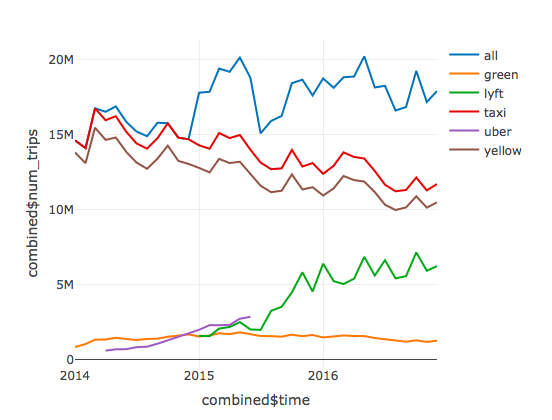
\includegraphics{figure/Num_trips_summary.png}
\caption{}
\end{figure}
\subsection{Yellow Taxi}\label{yellow-taxi-2}

The total size of all yellow taxi trip data CSV files (from Jan 2010 to
Dec 2016) is 191.38 GB, and NYC yellow taxi trip data from Jan 2009 to
the most recent month can be found on NYC Taxi \& Limousine Commission
(TLC). The data were collected and provided to the NYC TLC by technology
providers authorized under the Taxicab \& Livery Passenger Enhancement
Programs (TPEP/LPEP).

The yellow taxi trip records include the following fields: pick-up and
drop-off dates/times, pick-up and drop-off locations, trip distances,
itemized fares, rate types, payment types, and driver-reported passenger
counts.

\subsection{Green Taxi}\label{green-taxi-2}

The total size of green taxi trip data CSV files (from Aug 2013 to Dec
2016) is 7.8 GB, and green taxi trip data from Aug 2013 to the most
recent month can be downloaded from NYC Taxi \& Limousine Commission
(TLC). The data were collected and provided to the NYC TLC by technology
providers authorized under the Taxicab \& Livery Passenger Enhancement
Programs (TPEP/LPEP).

The green taxi trip records include the following fields: pick-up and
drop-off dates/times, pick-up and drop-off locations, trip distances,
itemized fares, rate types, payment types, and driver-reported passenger
counts.

\subsection{Uber}\label{uber-2}

The total size of Uber pick-up data (over 4.5 million from Apr to Sep
2014 and 14.3 million from Jan to June 2015) is 4.3 MB, and thanks to
FiveThirtyEight who obtained the data from NYC TLC by submitting a
Freedom of Information Law request on July 20, 2015, these data are now
open to public.

The 2014 Uber data contains four variables: Data/Time (the date and time
of the Uber pick-up), Lat (the latitude of the Uber pick-up), Lon (the
longitude of the Uber pick-up), and Base (the TLC base company code
affiliated with the Uber pickup).

The 2015 Uber data contains four variables: Dispatching\_base\_num (the
TLC base company code of the base that dispatched the Uber),
Pickup\_date (the date of the Uber pick-up), Affiliated\_base\_num (the
TLC base company code affiliated with the Uber pickup), and locationID
(the pick-up location ID affiliated with the Uber pickup).

\subsection{Lyft}\label{lyft-2}

The total size of weely-aggregated Lyft trip data (from Jan 2015 to Dec
2016) is 914.9 MB, and these data are open to public and
weekly-aggregated Lyft data from 2015 to the most recent week can be
found on NYC OpenData website.

\subsection{Storage}\label{storage}

The total size of all CSV files of the four services is about 200 GB,
and a laptop usually has memory less than or equal to 8GB. Limited
memory constrains the amount of data that can be loaded by a personal
computer. When users load data into R environment, R keeps them in
memory; when the amount of data loaded into R environment gets close to
the limit of a computer's memory, R becomes unresponsive or force quit
the current session. Therefore, better ways to work with data that takes
more space than 8 GB is needed. According to Weijia Zhang (2016),
comparing to RAM, hard disk is often used to store medium-sized data,
because it is affordable and are designed for storing large items
permanently. However, retrieving data from hard drives usually takes
about 1,000,000 times more time.

\section{ETL nyctaxi Package}\label{etl-nyctaxi-package}

etl is the parent package of nyctaxi. etl package provides a
CRAN-friendly framework that allows R users to work with medium data
without any knowledge in SQL database. The end result is a populated SQL
database, but the user interaction takes place solely within R. It has
three operations -extract, transfer, and load- which bring real-time
data into local or remote databases. etl-dependent packages make medium
data - too big to store in memory on a laptop- more accessible to a
wider audience. Additionally, etl-dependent packages use SQL translation
supported by dyplr.

nyctaxi was initially designed to work with New York City taxi data, but
later on Uber and Lyft data were added and the ETL functions are
modified to be specialized in working with these data. This package
compiled three major sources of hail service in New York City so that it
is convenient for users to compare and contrast the performance of these
three services.

This package inherits functions from many packages: etl, dplyr, DBI,
rlang, and stringr. Since SQL databases are good tools for medium data
analysis, ETL functions build connection to a SQL database at the back
end and convert R code automatically into SQL queries and send them to
the SQL database to get data tables containing data of each hail
service. Thus, users do not need to have any knowledge of SQL queries
and they can draw in any subsets of the data from the SQL database in R.

In general, extract.nyctaxi function download data of the four types of
hail service data (yellow taxi, green taxi, uber, and lyft) from the
corresponding sources. transform.nyctaxi uses different techniques to
clean all four types of data to get then ready for the next step.
extract.load loads the data user selected to a SQL database.

nyctaxi lives on the Comprehensive R Archive Network (CRAN), and
Packages can be installed with the install.packages() function in R.
\begin{Shaded}
\begin{Highlighting}[]
\CommentTok{#install the package}
\KeywordTok{install.packages}\NormalTok{(}\StringTok{"nyctaxi"}\NormalTok{)}

\CommentTok{# load the package}
\KeywordTok{library}\NormalTok{(nyctaxi)}
\end{Highlighting}
\end{Shaded}
Users need to create an etl object in order to apply the etl operations
to it, and only the name of the SQL database, working directory, and
type of SQL database need to be specified during initialization. If the
type of SQL database is not specified, a local RSQLite database will be
generated as default.
\begin{Shaded}
\begin{Highlighting}[]
\CommentTok{# initializing an etl object}
\NormalTok{db <-}\StringTok{ }\KeywordTok{src_mysql}\NormalTok{(}\StringTok{"nyctaxi"}\NormalTok{, }\DataTypeTok{user =} \StringTok{"urname"}\NormalTok{, }\DataTypeTok{host =} \StringTok{"host"}\NormalTok{, }\DataTypeTok{password =} \StringTok{"pw"}\NormalTok{)}
\NormalTok{taxi <-}\StringTok{ }\KeywordTok{etl}\NormalTok{(}\StringTok{"nyctaxi"}\NormalTok{, }\DataTypeTok{dir =} \StringTok{"~/Desktop/nyctaxi"}\NormalTok{, db)}
\end{Highlighting}
\end{Shaded}
In the example above, a folder called nyctaxi is created on the desktop
and a connection to a MySQL database is generated. In the procession of
initialization, a local folder contains two subfolders, \texttt{raw} and
\texttt{load}, are also created under the directory the user specifies.
\texttt{raw} folder stores data downloaded from online open sources, and
\texttt{load} folder stores cleaned CSV data files that are ready to be
loaded into SQL database. The ETL framework keeps data directly scraped
from online data sources in their original forms. In this way, the
original data is always available to users in case data corruption
happens in later stages.

After an etl object is created (nyctaxi is the etl object in this case),
four parameters are needed to specify the data that users want: (1) obj:
an etl object (2) years: a numeric vector giving the years. The default
is the most recent year. (3) months: a numeric vector giving the months.
The default is January to December. (4) type: a character variable
giving the type of data the user wants to download. There are four
types: yellow, green, uber, and lyft. The default is yellow.

\subsection{Taxi zone shapefile attached to nyctaxi R
package}\label{taxi-zone-shapefile-attached-to-nyctaxi-r-package}

\section{Extract}\label{extract}

etl\_extract.nyctaxi allows users to download New York City yellow taxi,
green taxi, Uber, and Lyft data that are specific to their month of
interest.

\subsection{Yellow Taxi}\label{yellow-taxi-3}

\subsection{Green Taxi}\label{green-taxi-3}

\subsection{Uber}\label{uber-3}

\subsection{Lyft}\label{lyft-3}

\section{Transform}\label{transform}

etl\_extract.nyctaxi allows users to transform New York City yellow
taxi, green taxi, Uber, and Lyft data into forms that are meaningful to
users.

\subsection{Yellow Taxi}\label{yellow-taxi-4}

\subsection{Green Taxi}\label{green-taxi-4}

\subsection{Uber}\label{uber-4}

\subsection{Lyft}\label{lyft-4}

\section{Load}\label{load}

etl\_extract.nyctaxi allows users to load New York City yellow taxi,
green taxi, Uber, and Lyft data into different data tables in a SQL
database.

\subsection{Yellow Taxi}\label{yellow-taxi-5}

\subsection{Green Taxi}\label{green-taxi-5}

\subsection{Uber}\label{uber-5}

\subsection{Lyft}\label{lyft-5}

\section{SQL Database Initialization}\label{sql-database-initialization}

\subsection{Yellow Taxi}\label{yellow-taxi-6}

\subsection{Green Taxi}\label{green-taxi-6}

\subsection{Uber}\label{uber-6}

\subsection{Lyft}\label{lyft-6}

\section{New Yoek City Hail Service
Summary}\label{new-yoek-city-hail-service-summary}

\section{Source Code}\label{source-code}

\subsection{ETL Extract}\label{etl-extract}
\begin{Shaded}
\begin{Highlighting}[]
\NormalTok{etl_extract.etl_nyctaxi <-}\StringTok{ }\ControlFlowTok{function}\NormalTok{(obj, }\DataTypeTok{years =} \KeywordTok{as.numeric}\NormalTok{(}\KeywordTok{format}\NormalTok{(}\KeywordTok{Sys.Date}\NormalTok{(),}\StringTok{'%Y'}\NormalTok{)), }
                                    \DataTypeTok{months =} \DecValTok{1}\OperatorTok{:}\DecValTok{12}\NormalTok{, }
                                    \DataTypeTok{type  =} \StringTok{"yellow"}\NormalTok{,...) \{}
  \CommentTok{#TAXI YELLOW-----------------------------------------------------------------------}
\NormalTok{  taxi_yellow <-}\StringTok{ }\ControlFlowTok{function}\NormalTok{(obj, years, months,...) \{}
    \KeywordTok{message}\NormalTok{(}\StringTok{"Extracting raw yellow taxi data..."}\NormalTok{)}
\NormalTok{    remote <-}\StringTok{ }\NormalTok{etl}\OperatorTok{::}\KeywordTok{valid_year_month}\NormalTok{(years, months, }\DataTypeTok{begin =} \StringTok{"2009-01-01"}\NormalTok{) }\OperatorTok
\StringTok{      }\KeywordTok{mutate_}\NormalTok{(}\DataTypeTok{src =} \OperatorTok{~}\KeywordTok{file.path}\NormalTok{(}\StringTok{"https://s3.amazonaws.com/nyc-tlc/trip+data"}\NormalTok{, }
                               \KeywordTok{paste0}\NormalTok{(}\StringTok{"yellow"}\NormalTok{, }\StringTok{"_tripdata_"}\NormalTok{, year, }\StringTok{"-"}\NormalTok{,}
\NormalTok{                                      stringr}\OperatorTok{::}\KeywordTok{str_pad}\NormalTok{(month, }\DecValTok{2}\NormalTok{, }\StringTok{"left"}\NormalTok{, }\StringTok{"0"}\NormalTok{), }\StringTok{".csv"}\NormalTok{))) }
    \KeywordTok{tryCatch}\NormalTok{(}\DataTypeTok{expr =}\NormalTok{ etl}\OperatorTok{::}\KeywordTok{smart_download}\NormalTok{(obj, remote}\OperatorTok{$}\NormalTok{src, ...),}
             \DataTypeTok{error =} \ControlFlowTok{function}\NormalTok{(e)\{}\KeywordTok{warning}\NormalTok{(e)\}, }
             \DataTypeTok{finally =} \KeywordTok{warning}\NormalTok{(}\StringTok{"Only the following data are availabel on TLC:}
\StringTok{                               Yellow taxi data: 2009 Jan - last month"}\NormalTok{))\} }
  \CommentTok{#TAXI GREEN-----------------------------------------------------------------------}
\NormalTok{  taxi_green <-}\StringTok{ }\ControlFlowTok{function}\NormalTok{(obj, years, months,...) \{}
    \KeywordTok{message}\NormalTok{(}\StringTok{"Extracting raw green taxi data..."}\NormalTok{)}
\NormalTok{    remote <-}\StringTok{ }\NormalTok{etl}\OperatorTok{::}\KeywordTok{valid_year_month}\NormalTok{(years, months, }\DataTypeTok{begin =} \StringTok{"2013-08-01"}\NormalTok{) }\OperatorTok
\StringTok{      }\KeywordTok{mutate_}\NormalTok{(}\DataTypeTok{src =} \OperatorTok{~}\KeywordTok{file.path}\NormalTok{(}\StringTok{"https://s3.amazonaws.com/nyc-tlc/trip+data"}\NormalTok{, }
                               \KeywordTok{paste0}\NormalTok{(}\StringTok{"green"}\NormalTok{, }\StringTok{"_tripdata_"}\NormalTok{, year, }\StringTok{"-"}\NormalTok{,}
\NormalTok{                                      stringr}\OperatorTok{::}\KeywordTok{str_pad}\NormalTok{(month, }\DecValTok{2}\NormalTok{, }\StringTok{"left"}\NormalTok{, }\StringTok{"0"}\NormalTok{), }\StringTok{".csv"}\NormalTok{)))}
    \KeywordTok{tryCatch}\NormalTok{(}\DataTypeTok{expr =}\NormalTok{ etl}\OperatorTok{::}\KeywordTok{smart_download}\NormalTok{(obj, remote}\OperatorTok{$}\NormalTok{src, ...),}
             \DataTypeTok{error =} \ControlFlowTok{function}\NormalTok{(e)\{}\KeywordTok{warning}\NormalTok{(e)\}, }
             \DataTypeTok{finally =} \KeywordTok{warning}\NormalTok{(}\StringTok{"Only the following data are availabel on TLC:}
\StringTok{                               Green taxi data: 2013 Aug - last month"}\NormalTok{))\} }
  \CommentTok{#UBER-----------------------------------------------------------------------}
\NormalTok{  uber <-}\StringTok{ }\ControlFlowTok{function}\NormalTok{(obj, years, months,...) \{}
    \KeywordTok{message}\NormalTok{(}\StringTok{"Extracting raw uber data..."}\NormalTok{)}
\NormalTok{    raw_month_}\DecValTok{2014}\NormalTok{ <-}\StringTok{ }\NormalTok{etl}\OperatorTok{::}\KeywordTok{valid_year_month}\NormalTok{(}\DataTypeTok{years =} \DecValTok{2014}\NormalTok{, }\DataTypeTok{months =} \DecValTok{4}\OperatorTok{:}\DecValTok{9}\NormalTok{)}
\NormalTok{    raw_month_}\DecValTok{2015}\NormalTok{ <-}\StringTok{ }\NormalTok{etl}\OperatorTok{::}\KeywordTok{valid_year_month}\NormalTok{(}\DataTypeTok{years =} \DecValTok{2015}\NormalTok{, }\DataTypeTok{months =} \DecValTok{1}\OperatorTok{:}\DecValTok{6}\NormalTok{)}
\NormalTok{    raw_month <-}\StringTok{ }\KeywordTok{bind_rows}\NormalTok{(raw_month_}\DecValTok{2014}\NormalTok{, raw_month_}\DecValTok{2015}\NormalTok{)}
\NormalTok{    path =}\StringTok{ "https://raw.githubusercontent.com/fivethirtyeight/uber-tlc-foil-response/master/uber-trip-data"}
\NormalTok{    remote <-}\StringTok{ }\NormalTok{etl}\OperatorTok{::}\KeywordTok{valid_year_month}\NormalTok{(years, months)}
\NormalTok{    remote_small <-}\StringTok{ }\KeywordTok{intersect}\NormalTok{(raw_month, remote)}
    \ControlFlowTok{if}\NormalTok{ (}\DecValTok{2015} \OperatorTok\StringTok{ }\NormalTok{remote_small}\OperatorTok{$}\NormalTok{year }\OperatorTok{&&}\StringTok{ }\OperatorTok{!}\NormalTok{(}\DecValTok{2014} \OperatorTok\StringTok{ }\NormalTok{remote_small}\OperatorTok{$}\NormalTok{year))\{}
      \CommentTok{#download 2015 data}
      \KeywordTok{message}\NormalTok{(}\StringTok{"Downloading Uber 2015 data..."}\NormalTok{)}
\NormalTok{      etl}\OperatorTok{::}\KeywordTok{smart_download}\NormalTok{(obj, }\StringTok{"https://github.com/fivethirtyeight/uber-tlc-foil-response/raw/master/uber-trip-data/uber-raw-data-janjune-15.csv.zip"}\NormalTok{,...)\}}
    \ControlFlowTok{else} \ControlFlowTok{if}\NormalTok{ (}\DecValTok{2015} \OperatorTok\StringTok{ }\NormalTok{remote_small}\OperatorTok{$}\NormalTok{year }\OperatorTok{&&}\StringTok{ }\DecValTok{2014} \OperatorTok\StringTok{ }\NormalTok{remote_small}\OperatorTok{$}\NormalTok{year) \{}
      \CommentTok{#download 2015 data}
      \KeywordTok{message}\NormalTok{(}\StringTok{"Downloading Uber 2015 data..."}\NormalTok{)}
\NormalTok{      etl}\OperatorTok{::}\KeywordTok{smart_download}\NormalTok{(obj, }\StringTok{"https://github.com/fivethirtyeight/uber-tlc-foil-response/raw/master/uber-trip-data/uber-raw-data-janjune-15.csv.zip"}\NormalTok{,...)}
      \CommentTok{#download 2014 data}
\NormalTok{      small <-}\StringTok{ }\NormalTok{remote_small }\OperatorTok
\StringTok{        }\KeywordTok{filter_}\NormalTok{(}\OperatorTok{~}\NormalTok{year }\OperatorTok{==}\StringTok{ }\DecValTok{2014}\NormalTok{) }\OperatorTok
\StringTok{        }\KeywordTok{mutate_}\NormalTok{(}\DataTypeTok{month_abb =} \OperatorTok{~}\KeywordTok{tolower}\NormalTok{(month.abb[month]),}
                \DataTypeTok{src =} \OperatorTok{~}\KeywordTok{file.path}\NormalTok{(path, }\KeywordTok{paste0}\NormalTok{(}\StringTok{"uber-raw-data-"}\NormalTok{,month_abb,}\KeywordTok{substr}\NormalTok{(year,}\DecValTok{3}\NormalTok{,}\DecValTok{4}\NormalTok{),}\StringTok{".csv"}\NormalTok{)))}
      \KeywordTok{message}\NormalTok{(}\StringTok{"Downloading Uber 2014 data..."}\NormalTok{)}
\NormalTok{      etl}\OperatorTok{::}\KeywordTok{smart_download}\NormalTok{(obj, small}\OperatorTok{$}\NormalTok{src,...) }
\NormalTok{    \} }\ControlFlowTok{else} \ControlFlowTok{if}\NormalTok{ (}\DecValTok{2014} \OperatorTok\StringTok{ }\NormalTok{remote_small}\OperatorTok{$}\NormalTok{year }\OperatorTok{&&}\StringTok{ }\OperatorTok{!}\NormalTok{(}\DecValTok{2015} \OperatorTok\StringTok{ }\NormalTok{remote_small}\OperatorTok{$}\NormalTok{year)) \{}
      \KeywordTok{message}\NormalTok{(}\StringTok{"Downloading Uber 2014 data..."}\NormalTok{)}
      \CommentTok{#file paths}
\NormalTok{      small <-}\StringTok{ }\NormalTok{remote_small }\OperatorTok
\StringTok{        }\KeywordTok{mutate_}\NormalTok{(}\DataTypeTok{month_abb =} \OperatorTok{~}\KeywordTok{tolower}\NormalTok{(month.abb[month]),}
                \DataTypeTok{src =} \OperatorTok{~}\KeywordTok{file.path}\NormalTok{(path, }\KeywordTok{paste0}\NormalTok{(}\StringTok{"uber-raw-data-"}\NormalTok{,month_abb,}\KeywordTok{substr}\NormalTok{(year,}\DecValTok{3}\NormalTok{,}\DecValTok{4}\NormalTok{),}\StringTok{".csv"}\NormalTok{)))}
\NormalTok{      etl}\OperatorTok{::}\KeywordTok{smart_download}\NormalTok{(obj, small}\OperatorTok{$}\NormalTok{src,...)\}}
    \ControlFlowTok{else}\NormalTok{ \{}\KeywordTok{warning}\NormalTok{(}\StringTok{"The Uber data you requested are not currently available. Only data from 2014/04-2014/09 and 2015/01-2015/06 are available..."}\NormalTok{)\}}
\NormalTok{    \} }
  \CommentTok{#LYFT-----------------------------------------------------------------------}
\NormalTok{  lyft <-}\StringTok{ }\ControlFlowTok{function}\NormalTok{(obj, years, months,...)\{}
    \KeywordTok{message}\NormalTok{(}\StringTok{"Extracting raw lyft data..."}\NormalTok{)}
    \CommentTok{#check if the week is valid}
\NormalTok{    valid_months <-}\StringTok{ }\NormalTok{etl}\OperatorTok{::}\KeywordTok{valid_year_month}\NormalTok{(years, months, }\DataTypeTok{begin =} \StringTok{"2015-01-01"}\NormalTok{)}
\NormalTok{    base_url =}\StringTok{ "https://data.cityofnewyork.us/resource/edp9-qgv4.csv"}
\NormalTok{    valid_months <-}\StringTok{ }\NormalTok{valid_months }\OperatorTok
\StringTok{      }\KeywordTok{mutate_}\NormalTok{(}\DataTypeTok{new_filenames =} \OperatorTok{~}\KeywordTok{paste0}\NormalTok{(}\StringTok{"lyft-"}\NormalTok{, year, }\StringTok{".csv"}\NormalTok{)) }\OperatorTok
\StringTok{      }\KeywordTok{mutate_}\NormalTok{(}\DataTypeTok{drop =} \OtherTok{TRUE}\NormalTok{)}
    \CommentTok{#only keep one data set per year}
\NormalTok{    year <-}\StringTok{ }\NormalTok{valid_months[}\DecValTok{1}\NormalTok{,}\DecValTok{1}\NormalTok{]}
\NormalTok{    n <-}\StringTok{ }\KeywordTok{nrow}\NormalTok{(valid_months)}
    \ControlFlowTok{for}\NormalTok{ (i }\ControlFlowTok{in} \DecValTok{2}\OperatorTok{:}\NormalTok{n) \{}
      \ControlFlowTok{if}\NormalTok{(year }\OperatorTok{==}\StringTok{ }\NormalTok{valid_months[i}\OperatorTok{-}\DecValTok{1}\NormalTok{,}\DecValTok{1}\NormalTok{]) \{}
\NormalTok{        valid_months[i,}\DecValTok{6}\NormalTok{] <-}\StringTok{ }\OtherTok{FALSE}
\NormalTok{        year <-}\StringTok{ }\NormalTok{valid_months[i}\OperatorTok{+}\DecValTok{1}\NormalTok{,}\DecValTok{1}\NormalTok{]}
\NormalTok{      \} }\ControlFlowTok{else}\NormalTok{ \{}
\NormalTok{        valid_months[i,}\DecValTok{6}\NormalTok{] <-}\StringTok{ }\OtherTok{TRUE}
\NormalTok{        year <-}\StringTok{ }\NormalTok{valid_months[i}\OperatorTok{+}\DecValTok{1}\NormalTok{,}\DecValTok{1}\NormalTok{]\}}
\NormalTok{      \}}
\NormalTok{    row_to_keep =}\StringTok{ }\NormalTok{valid_months}\OperatorTok{$}\NormalTok{drop}
\NormalTok{    valid_months <-}\StringTok{ }\NormalTok{valid_months[row_to_keep,]}
    
    \CommentTok{#download lyft files, try two different methods}
\NormalTok{    first_try<-}\KeywordTok{tryCatch}\NormalTok{(}
      \KeywordTok{download_nyc_data}\NormalTok{(obj, base_url, valid_months}\OperatorTok{$}\NormalTok{year, }\DataTypeTok{n =} \DecValTok{50000}\NormalTok{,}
                        \DataTypeTok{names =}\NormalTok{ valid_months}\OperatorTok{$}\NormalTok{new_filenames),}
      \DataTypeTok{error =} \ControlFlowTok{function}\NormalTok{(e)\{}\KeywordTok{warning}\NormalTok{(e)\},}\DataTypeTok{finally =} \StringTok{'method = "libcurl" fails'}\NormalTok{)}
\NormalTok{  \}}
  
  \ControlFlowTok{if}\NormalTok{ (type }\OperatorTok{==}\StringTok{ "yellow"}\NormalTok{)\{}\KeywordTok{taxi_yellow}\NormalTok{(obj, years, months,...)\} }
  \ControlFlowTok{else} \ControlFlowTok{if}\NormalTok{ (type }\OperatorTok{==}\StringTok{ "green"}\NormalTok{)\{}\KeywordTok{taxi_green}\NormalTok{(obj, years, months,...)\}}
  \ControlFlowTok{else} \ControlFlowTok{if}\NormalTok{ (type }\OperatorTok{==}\StringTok{ "uber"}\NormalTok{)\{}\KeywordTok{uber}\NormalTok{(obj, years, months,...)\}}
  \ControlFlowTok{else} \ControlFlowTok{if}\NormalTok{ (type }\OperatorTok{==}\StringTok{ "lyft"}\NormalTok{)\{}\KeywordTok{lyft}\NormalTok{(obj, years, months,...)\}}
  \ControlFlowTok{else}\NormalTok{ \{}\KeywordTok{message}\NormalTok{(}\StringTok{"The type you chose does not exit..."}\NormalTok{)\}}
  
  \KeywordTok{invisible}\NormalTok{(obj)}
\NormalTok{\}}
\end{Highlighting}
\end{Shaded}
\subsection{ETL Transform}\label{etl-transform}
\begin{Shaded}
\begin{Highlighting}[]
\NormalTok{etl_transform.etl_nyctaxi <-}\StringTok{ }\ControlFlowTok{function}\NormalTok{(obj, }\DataTypeTok{years =} \KeywordTok{as.numeric}\NormalTok{(}\KeywordTok{format}\NormalTok{(}\KeywordTok{Sys.Date}\NormalTok{(),}\StringTok{'%Y'}\NormalTok{)), }
                                    \DataTypeTok{months =} \DecValTok{1}\OperatorTok{:}\DecValTok{12}\NormalTok{, }
                                    \DataTypeTok{type  =} \StringTok{"yellow"}\NormalTok{,...) \{}
  \CommentTok{#TAXI YELLOW----------------------------------------------------------------}
\NormalTok{  taxi_yellow <-}\StringTok{ }\ControlFlowTok{function}\NormalTok{(obj, years, months) \{}
    \KeywordTok{message}\NormalTok{(}\StringTok{"Transforming yellow taxi data from raw to load directory..."}\NormalTok{)}
    \CommentTok{#create a df of file path of the files that the user wants to transform}
\NormalTok{    remote <-}\StringTok{ }\NormalTok{etl}\OperatorTok{::}\KeywordTok{valid_year_month}\NormalTok{(years, months, }\DataTypeTok{begin =} \StringTok{"2009-01-01"}\NormalTok{) }\OperatorTok
\StringTok{      }\KeywordTok{mutate_}\NormalTok{(}\DataTypeTok{src =} \OperatorTok{~}\KeywordTok{file.path}\NormalTok{(}\KeywordTok{attr}\NormalTok{(obj, }\StringTok{"raw_dir"}\NormalTok{), }
                               \KeywordTok{paste0}\NormalTok{(}\StringTok{"yellow"}\NormalTok{, }\StringTok{"_tripdata_"}\NormalTok{, year, }\StringTok{"-"}\NormalTok{,}
\NormalTok{                                      stringr}\OperatorTok{::}\KeywordTok{str_pad}\NormalTok{(month, }\DecValTok{2}\NormalTok{, }\StringTok{"left"}\NormalTok{, }\StringTok{"0"}\NormalTok{), }\StringTok{".csv"}\NormalTok{))) }
    \CommentTok{#create a df of file path of the files that are in the raw directory}
\NormalTok{    src <-}\StringTok{ }\KeywordTok{list.files}\NormalTok{(}\KeywordTok{attr}\NormalTok{(obj, }\StringTok{"raw_dir"}\NormalTok{), }\StringTok{"yellow"}\NormalTok{, }\DataTypeTok{full.names =} \OtherTok{TRUE}\NormalTok{)}
\NormalTok{    src_small <-}\StringTok{ }\KeywordTok{intersect}\NormalTok{(src, remote}\OperatorTok{$}\NormalTok{src)}
    \CommentTok{#Move the files}
\NormalTok{    in_raw <-}\StringTok{ }\KeywordTok{basename}\NormalTok{(src_small)}
\NormalTok{    in_load <-}\StringTok{ }\KeywordTok{basename}\NormalTok{(}\KeywordTok{list.files}\NormalTok{(}\KeywordTok{attr}\NormalTok{(obj, }\StringTok{"load_dir"}\NormalTok{), }\StringTok{"yellow"}\NormalTok{, }\DataTypeTok{full.names =} \OtherTok{TRUE}\NormalTok{))}
\NormalTok{    file_remian <-}\StringTok{ }\KeywordTok{setdiff}\NormalTok{(in_raw,in_load)}
    \KeywordTok{file.copy}\NormalTok{(}\KeywordTok{file.path}\NormalTok{(}\KeywordTok{attr}\NormalTok{(obj, }\StringTok{"raw_dir"}\NormalTok{),file_remian),}
              \KeywordTok{file.path}\NormalTok{(}\KeywordTok{attr}\NormalTok{(obj, }\StringTok{"load_dir"}\NormalTok{),file_remian) )\}}
  \CommentTok{#TAXI GREEN----------------------------------------------------------------}
\NormalTok{  taxi_green <-}\StringTok{ }\ControlFlowTok{function}\NormalTok{(obj, years, months) \{}
    \KeywordTok{message}\NormalTok{(}\StringTok{"Transforming green taxi data from raw to load directory..."}\NormalTok{)}
    \CommentTok{#create a df of file path of the files that the user wants to transform}
\NormalTok{    remote <-}\StringTok{ }\NormalTok{etl}\OperatorTok{::}\KeywordTok{valid_year_month}\NormalTok{(years, months, }\DataTypeTok{begin =} \StringTok{"2013-08-01"}\NormalTok{) }\OperatorTok
\StringTok{      }\KeywordTok{mutate_}\NormalTok{(}\DataTypeTok{src =} \OperatorTok{~}\KeywordTok{file.path}\NormalTok{(}\KeywordTok{attr}\NormalTok{(obj, }\StringTok{"raw_dir"}\NormalTok{), }\KeywordTok{paste0}\NormalTok{(}\StringTok{"green"}\NormalTok{, }\StringTok{"_tripdata_"}\NormalTok{, year, }\StringTok{"-"}\NormalTok{,}
\NormalTok{                                      stringr}\OperatorTok{::}\KeywordTok{str_pad}\NormalTok{(month, }\DecValTok{2}\NormalTok{, }\StringTok{"left"}\NormalTok{, }\StringTok{"0"}\NormalTok{), }\StringTok{".csv"}\NormalTok{))) }
    \CommentTok{#create a df of file path of the files that are in the raw directory}
\NormalTok{    src <-}\StringTok{ }\KeywordTok{list.files}\NormalTok{(}\KeywordTok{attr}\NormalTok{(obj, }\StringTok{"raw_dir"}\NormalTok{), }\StringTok{"green"}\NormalTok{, }\DataTypeTok{full.names =} \OtherTok{TRUE}\NormalTok{)}
\NormalTok{    src_small <-}\StringTok{ }\KeywordTok{intersect}\NormalTok{(src, remote}\OperatorTok{$}\NormalTok{src)}
    \CommentTok{#Clean the green taxi data files}
    \CommentTok{#get rid of 2nd blank row----------------------------------------------------------}
    \ControlFlowTok{if}\NormalTok{ (}\KeywordTok{length}\NormalTok{(src_small) }\OperatorTok{==}\StringTok{ }\DecValTok{0}\NormalTok{)\{}
      \KeywordTok{message}\NormalTok{(}\StringTok{"The files you requested are not available in the raw directory."}\NormalTok{)}
\NormalTok{    \} }\ControlFlowTok{else}\NormalTok{\{}
      \CommentTok{#a list of the ones that have a 2nd blank row}
\NormalTok{      remote_green_}\DecValTok{1}\NormalTok{ <-}\StringTok{ }\NormalTok{remote }\OperatorTok\StringTok{ }\KeywordTok{filter_}\NormalTok{(}\OperatorTok{~}\NormalTok{year }\OperatorTok{!=}\StringTok{ }\DecValTok{2015}\NormalTok{)}
\NormalTok{      src_small_green_}\DecValTok{1}\NormalTok{ <-}\StringTok{ }\KeywordTok{intersect}\NormalTok{(src, remote_green_}\DecValTok{1}\OperatorTok{$}\NormalTok{src)}
      \CommentTok{# check that the sys support command line, and then remove the blank 2nd row}
      \ControlFlowTok{if}\NormalTok{(}\KeywordTok{length}\NormalTok{(src_small_green_}\DecValTok{1}\NormalTok{) }\OperatorTok{!=}\StringTok{ }\DecValTok{0}\NormalTok{) \{}
        \ControlFlowTok{if}\NormalTok{ (.Platform}\OperatorTok{$}\NormalTok{OS.type }\OperatorTok{==}\StringTok{ "unix"}\NormalTok{)\{}
\NormalTok{          cmds_}\DecValTok{1}\NormalTok{ <-}\StringTok{ }\KeywordTok{paste}\NormalTok{(}\StringTok{"sed -i -e '2d'"}\NormalTok{, src_small_green_}\DecValTok{1}\NormalTok{)}
          \KeywordTok{lapply}\NormalTok{(cmds_}\DecValTok{1}\NormalTok{, system)}
\NormalTok{        \} }\ControlFlowTok{else}\NormalTok{ \{}
          \KeywordTok{message}\NormalTok{(}\StringTok{"Windows system does not currently support removing the 2nd blank row }
\StringTok{                  in the green taxi datasets. This might affect loading data into SQL..."}\NormalTok{)\}}
\NormalTok{        \}}\ControlFlowTok{else}\NormalTok{ \{}
          \StringTok{"You did not request for any green taxi data, or all the green taxi data you requested are cleaned."}\NormalTok{\}}
      \CommentTok{#fix column number---------------------------------------------------------------}
\NormalTok{      remote_green_}\DecValTok{2}\NormalTok{ <-}\StringTok{ }\NormalTok{remote }\OperatorTok
\StringTok{        }\KeywordTok{filter_}\NormalTok{(}\OperatorTok{~}\NormalTok{year }\OperatorTok\StringTok{ }\KeywordTok{c}\NormalTok{(}\DecValTok{2013}\NormalTok{, }\DecValTok{2014}\NormalTok{, }\DecValTok{2015}\NormalTok{)) }\OperatorTok
\StringTok{        }\KeywordTok{mutate_}\NormalTok{(}\DataTypeTok{keep =} \OperatorTok{~}\KeywordTok{ifelse}\NormalTok{(year }\OperatorTok\StringTok{ }\KeywordTok{c}\NormalTok{(}\DecValTok{2013}\NormalTok{,}\DecValTok{2014}\NormalTok{), }\DecValTok{20}\NormalTok{,}\DecValTok{21}\NormalTok{),}
                \DataTypeTok{new_file =} \OperatorTok{~}\KeywordTok{paste0}\NormalTok{(}\StringTok{"green_tripdata_"}\NormalTok{, year, }\StringTok{"_"}\NormalTok{, }
\NormalTok{                                   stringr}\OperatorTok{::}\KeywordTok{str_pad}\NormalTok{(month, }\DecValTok{2}\NormalTok{, }\StringTok{"left"}\NormalTok{, }\StringTok{"0"}\NormalTok{),}
                                   \StringTok{".csv"}\NormalTok{))}
\NormalTok{      src_small_green_}\DecValTok{2}\NormalTok{ <-}\StringTok{ }\KeywordTok{intersect}\NormalTok{(src, remote_green_}\DecValTok{2}\OperatorTok{$}\NormalTok{src)}
\NormalTok{      src_small_green_2_df <-}\StringTok{ }\KeywordTok{data.frame}\NormalTok{(src_small_green_}\DecValTok{2}\NormalTok{) }
      \KeywordTok{names}\NormalTok{(src_small_green_2_df) <-}\StringTok{ "src"}
\NormalTok{      src_small_green_2_df <-}\StringTok{ }\KeywordTok{inner_join}\NormalTok{(src_small_green_2_df, remote_green_}\DecValTok{2}\NormalTok{, }\DataTypeTok{by =} \StringTok{"src"}\NormalTok{)}
\NormalTok{      src_small_green_2_df <-}\StringTok{ }\NormalTok{src_small_green_2_df }\OperatorTok
\StringTok{        }\KeywordTok{mutate}\NormalTok{(}\DataTypeTok{cmds_2 =} \KeywordTok{paste}\NormalTok{(}\StringTok{"cut -d, -f1-"}\NormalTok{, keep,}\StringTok{" "}\NormalTok{,src, }\StringTok{" > "}\NormalTok{,}\KeywordTok{attr}\NormalTok{(obj, }\StringTok{"raw_dir"}\NormalTok{),}\StringTok{"/green_tripdata_"}\NormalTok{, }
\NormalTok{                              year, }\StringTok{"_"}\NormalTok{, stringr}\OperatorTok{::}\KeywordTok{str_pad}\NormalTok{(month, }\DecValTok{2}\NormalTok{, }\StringTok{"left"}\NormalTok{, }\StringTok{"0"}\NormalTok{),}\StringTok{".csv"}\NormalTok{, }\DataTypeTok{sep =} \StringTok{""}\NormalTok{))}
      \CommentTok{#remove the extra column}
      \ControlFlowTok{if}\NormalTok{(}\KeywordTok{length}\NormalTok{(src_small_green_}\DecValTok{2}\NormalTok{) }\OperatorTok{!=}\StringTok{ }\DecValTok{0}\NormalTok{) \{}
        \ControlFlowTok{if}\NormalTok{ (.Platform}\OperatorTok{$}\NormalTok{OS.type }\OperatorTok{==}\StringTok{ "unix"}\NormalTok{)\{}
          \KeywordTok{lapply}\NormalTok{(src_small_green_2_df}\OperatorTok{$}\NormalTok{cmds_}\DecValTok{2}\NormalTok{, system)\} }
        \ControlFlowTok{else}\NormalTok{ \{}
          \KeywordTok{message}\NormalTok{(}\StringTok{"Windows system does not currently support removing the 2nd blank row }
\StringTok{                  in the green taxi datasets. This might affect loading data into SQL..."}\NormalTok{)\}}
\NormalTok{        \}}\ControlFlowTok{else}\NormalTok{ \{}
          \StringTok{"All the green taxi data you requested are in cleaned formats."}\NormalTok{\}}
      \CommentTok{#Find the files paths of the files that need to be transformed----------------------}
      \KeywordTok{file.rename}\NormalTok{(}\KeywordTok{file.path}\NormalTok{(}\KeywordTok{dirname}\NormalTok{(src_small_green_2_df}\OperatorTok{$}\NormalTok{src),}
\NormalTok{                            src_small_green_2_df}\OperatorTok{$}\NormalTok{new_file), }
                  \KeywordTok{file.path}\NormalTok{(}\KeywordTok{attr}\NormalTok{(obj, }\StringTok{"load_dir"}\NormalTok{), }\KeywordTok{basename}\NormalTok{(src_small_green_2_df}\OperatorTok{$}\NormalTok{src)))}
      \CommentTok{#Move the files}
\NormalTok{      in_raw <-}\StringTok{ }\KeywordTok{basename}\NormalTok{(src_small)}
\NormalTok{      in_load <-}\StringTok{ }\KeywordTok{basename}\NormalTok{(}\KeywordTok{list.files}\NormalTok{(}\KeywordTok{attr}\NormalTok{(obj, }\StringTok{"load_dir"}\NormalTok{), }\StringTok{"green"}\NormalTok{, }\DataTypeTok{full.names =} \OtherTok{TRUE}\NormalTok{))}
\NormalTok{      file_remian <-}\StringTok{ }\KeywordTok{setdiff}\NormalTok{(in_raw,in_load)}
      \KeywordTok{file.copy}\NormalTok{(}\KeywordTok{file.path}\NormalTok{(}\KeywordTok{attr}\NormalTok{(obj, }\StringTok{"raw_dir"}\NormalTok{),file_remian), }\KeywordTok{file.path}\NormalTok{(}\KeywordTok{attr}\NormalTok{(obj, }\StringTok{"load_dir"}\NormalTok{),file_remian) )\}\}}
  \CommentTok{#UBER----------------------------------------------------------------}
\NormalTok{  uber <-}\StringTok{ }\ControlFlowTok{function}\NormalTok{(obj) \{}
    \KeywordTok{message}\NormalTok{(}\StringTok{"Transforming uber data from raw to load directory..."}\NormalTok{)}
    \CommentTok{#creat a list of 2014 uber data file directory}
\NormalTok{    uber14_list <-}\StringTok{ }\KeywordTok{list.files}\NormalTok{(}\DataTypeTok{path =} \KeywordTok{attr}\NormalTok{(obj, }\StringTok{"raw_dir"}\NormalTok{), }\DataTypeTok{pattern =} \StringTok{"14.csv"}\NormalTok{)}
\NormalTok{    uber14_list <-}\StringTok{ }\KeywordTok{data.frame}\NormalTok{(uber14_list)}
\NormalTok{    uber14_list <-}\StringTok{ }\NormalTok{uber14_list }\OperatorTok\StringTok{ }\KeywordTok{mutate_}\NormalTok{(}\DataTypeTok{file_path =} \OperatorTok{~}\KeywordTok{file.path}\NormalTok{(}\KeywordTok{attr}\NormalTok{(obj, }\StringTok{"raw_dir"}\NormalTok{), uber14_list))}
\NormalTok{    uber14file <-}\StringTok{ }\KeywordTok{lapply}\NormalTok{(uber14_list}\OperatorTok{$}\NormalTok{file_path, readr}\OperatorTok{::}\NormalTok{read_csv)}
\NormalTok{    n <-}\StringTok{ }\KeywordTok{length}\NormalTok{(uber14file)}
    \ControlFlowTok{if}\NormalTok{ (n }\OperatorTok{==}\StringTok{ }\DecValTok{1}\NormalTok{) \{}
\NormalTok{      uber14 <-}\StringTok{ }\KeywordTok{data.frame}\NormalTok{(uber14file[}\DecValTok{1}\NormalTok{])}
\NormalTok{    \} }\ControlFlowTok{else} \ControlFlowTok{if}\NormalTok{ (n }\OperatorTok{==}\StringTok{ }\DecValTok{2}\NormalTok{) \{}
\NormalTok{      uber14 <-}\StringTok{ }\KeywordTok{bind_rows}\NormalTok{(uber14file[}\DecValTok{1}\NormalTok{], uber14file[}\DecValTok{2}\NormalTok{])}
\NormalTok{    \} }\ControlFlowTok{else} \ControlFlowTok{if}\NormalTok{ (n }\OperatorTok{>}\StringTok{ }\DecValTok{2}\NormalTok{) \{}
\NormalTok{      uber14 <-}\StringTok{ }\KeywordTok{bind_rows}\NormalTok{(uber14file[}\DecValTok{1}\NormalTok{], uber14file[}\DecValTok{2}\NormalTok{])}
      \ControlFlowTok{for}\NormalTok{ (i }\ControlFlowTok{in} \DecValTok{3}\OperatorTok{:}\NormalTok{n)\{uber14 <-}\StringTok{ }\KeywordTok{bind_rows}\NormalTok{(uber14, uber14file[i])\}}
\NormalTok{    \}}
\NormalTok{    substrRight <-}\StringTok{ }\ControlFlowTok{function}\NormalTok{(x, n)\{}\KeywordTok{substr}\NormalTok{(x, }\KeywordTok{nchar}\NormalTok{(x)}\OperatorTok{-}\NormalTok{n}\OperatorTok{+}\DecValTok{1}\NormalTok{, }\KeywordTok{nchar}\NormalTok{(x))\}}
\NormalTok{    uber14_datetime <-}\StringTok{ }\NormalTok{uber14 }\OperatorTok
\StringTok{      }\KeywordTok{mutate}\NormalTok{(}\DataTypeTok{date =} \KeywordTok{gsub}\NormalTok{( }\StringTok{" .*$"}\NormalTok{, }\StringTok{""}\NormalTok{, }\StringTok{`}\DataTypeTok{Date/Time}\StringTok{`}\NormalTok{), }\DataTypeTok{len_date =} \KeywordTok{nchar}\NormalTok{(date), }
             \DataTypeTok{time =} \KeywordTok{sub}\NormalTok{(}\StringTok{'.*}\CharTok{\textbackslash{}\textbackslash{}}\StringTok{ '}\NormalTok{, }\StringTok{''}\NormalTok{, }\StringTok{`}\DataTypeTok{Date/Time}\StringTok{`}\NormalTok{))}
\NormalTok{    uber14_datetime <-}\StringTok{ }\NormalTok{uber14_datetime }\OperatorTok
\StringTok{      }\KeywordTok{mutate}\NormalTok{(}\DataTypeTok{month =} \KeywordTok{substr}\NormalTok{(}\StringTok{`}\DataTypeTok{Date/Time}\StringTok{`}\NormalTok{, }\DecValTok{1}\NormalTok{, }\DecValTok{1}\NormalTok{),}
             \DataTypeTok{day =} \KeywordTok{ifelse}\NormalTok{(len_date }\OperatorTok{==}\StringTok{ }\DecValTok{8}\NormalTok{, }\KeywordTok{substr}\NormalTok{(}\StringTok{`}\DataTypeTok{Date/Time}\StringTok{`}\NormalTok{, }\DecValTok{3}\NormalTok{,}\DecValTok{3}\NormalTok{),}\KeywordTok{substr}\NormalTok{(}\StringTok{`}\DataTypeTok{Date/Time}\StringTok{`}\NormalTok{, }\DecValTok{3}\NormalTok{,}\DecValTok{4}\NormalTok{)),}
             \DataTypeTok{pickup_date =}\NormalTok{ lubridate}\OperatorTok{::}\KeywordTok{ymd_hms}\NormalTok{(}\KeywordTok{paste0}\NormalTok{(}\StringTok{"2014-"}\NormalTok{, month, }\StringTok{"-"}\NormalTok{, day, }\StringTok{" "}\NormalTok{, time)))}
\NormalTok{    uber14_df <-}\StringTok{ }\NormalTok{uber14_datetime[}\OperatorTok{-}\KeywordTok{c}\NormalTok{(}\DecValTok{1}\NormalTok{,}\DecValTok{5}\OperatorTok{:}\DecValTok{9}\NormalTok{)]}
    
    \CommentTok{#2015}
\NormalTok{    zipped_uberfileURL <-}\StringTok{ }\KeywordTok{file.path}\NormalTok{(}\KeywordTok{attr}\NormalTok{(obj, }\StringTok{"raw_dir"}\NormalTok{), }\StringTok{"uber-raw-data-janjune-15.csv.zip"}\NormalTok{)}
\NormalTok{    raw_month_}\DecValTok{2015}\NormalTok{ <-}\StringTok{ }\NormalTok{etl}\OperatorTok{::}\KeywordTok{valid_year_month}\NormalTok{(}\DataTypeTok{years =} \DecValTok{2015}\NormalTok{, }\DataTypeTok{months =} \DecValTok{1}\OperatorTok{:}\DecValTok{6}\NormalTok{)}
\NormalTok{    remote_}\DecValTok{2015}\NormalTok{ <-}\StringTok{ }\NormalTok{etl}\OperatorTok{::}\KeywordTok{valid_year_month}\NormalTok{(years, months)}
\NormalTok{    remote_small_}\DecValTok{2015}\NormalTok{ <-}\StringTok{ }\KeywordTok{inner_join}\NormalTok{(raw_month_}\DecValTok{2015}\NormalTok{, remote_}\DecValTok{2015}\NormalTok{)}
    \ControlFlowTok{if}\NormalTok{(}\KeywordTok{file.exists}\NormalTok{(zipped_uberfileURL) }\OperatorTok{&&}\StringTok{ }\KeywordTok{nrow}\NormalTok{(remote_small_}\DecValTok{2015}\NormalTok{) }\OperatorTok{!=}\StringTok{ }\DecValTok{0}\NormalTok{)\{}
\NormalTok{      utils}\OperatorTok{::}\KeywordTok{unzip}\NormalTok{(}\DataTypeTok{zipfile =}\NormalTok{ zipped_uberfileURL, }
                   \DataTypeTok{unzip =} \StringTok{"internal"}\NormalTok{,}
                   \DataTypeTok{exdir =} \KeywordTok{file.path}\NormalTok{(}\KeywordTok{tempdir}\NormalTok{(), }\StringTok{"uber-raw-data-janjune-15.csv.zip"}\NormalTok{))}
\NormalTok{      uber15 <-}\StringTok{ }\NormalTok{readr}\OperatorTok{::}\KeywordTok{read_csv}\NormalTok{(}\KeywordTok{file.path}\NormalTok{(}\KeywordTok{tempdir}\NormalTok{(), }\StringTok{"uber-raw-data-janjune-15.csv.zip"}\NormalTok{,}\StringTok{"uber-raw-data-janjune-15.csv"}\NormalTok{))\}}
    
    \KeywordTok{names}\NormalTok{(uber14_df) <-}\StringTok{ }\KeywordTok{c}\NormalTok{(}\StringTok{"lat"}\NormalTok{, }\StringTok{"lon"}\NormalTok{, }\StringTok{"affiliated_base_num"}\NormalTok{, }\StringTok{"pickup_date"}\NormalTok{)}
    \KeywordTok{names}\NormalTok{(uber15) <-}\StringTok{ }\KeywordTok{tolower}\NormalTok{(}\KeywordTok{names}\NormalTok{(uber15))}
\NormalTok{    uber <-}\StringTok{ }\KeywordTok{bind_rows}\NormalTok{(uber14_df, uber15)}
\NormalTok{    utils}\OperatorTok{::}\KeywordTok{write.csv}\NormalTok{(uber, }\KeywordTok{file.path}\NormalTok{(}\KeywordTok{tempdir}\NormalTok{() ,}\StringTok{"uber.csv"}\NormalTok{))}
    \ControlFlowTok{if}\NormalTok{(}\KeywordTok{nrow}\NormalTok{(uber) }\OperatorTok{!=}\StringTok{ }\DecValTok{0}\NormalTok{) \{}
      \ControlFlowTok{if}\NormalTok{ (.Platform}\OperatorTok{$}\NormalTok{OS.type }\OperatorTok{==}\StringTok{ "unix"}\NormalTok{)\{}
\NormalTok{        cmds_}\DecValTok{3}\NormalTok{ <-}\StringTok{ }\KeywordTok{paste}\NormalTok{(}\StringTok{"cut -d, -f2-7 "}\NormalTok{,}\KeywordTok{file.path}\NormalTok{(}\KeywordTok{tempdir}\NormalTok{(),}\StringTok{"uber.csv"}\NormalTok{), }\StringTok{" > "}\NormalTok{, }\KeywordTok{file.path}\NormalTok{(}\KeywordTok{attr}\NormalTok{(obj, }\StringTok{"load_dir"}\NormalTok{),}\StringTok{"uber.csv"}\NormalTok{))}
        \KeywordTok{lapply}\NormalTok{(cmds_}\DecValTok{3}\NormalTok{, system)}
\NormalTok{      \} }\ControlFlowTok{else}\NormalTok{ \{}
        \KeywordTok{message}\NormalTok{(}\StringTok{"Windows system does not currently support removing the 2nd blank row }
\StringTok{                in the green taxi datasets. This might affect loading data into SQL..."}\NormalTok{)\}}
\NormalTok{      \}}\ControlFlowTok{else}\NormalTok{ \{}
        \StringTok{"You did not request for any green taxi data, or all the green taxi data you requested are cleaned."}\NormalTok{\}}
\NormalTok{    \}}
  \CommentTok{#LYFT----------------------------------------------------------------}
\NormalTok{  lyft <-}\StringTok{ }\ControlFlowTok{function}\NormalTok{(obj, years, months)\{}
\NormalTok{    valid_months <-}\StringTok{ }\NormalTok{etl}\OperatorTok{::}\KeywordTok{valid_year_month}\NormalTok{(years, }\DataTypeTok{months =} \DecValTok{1}\NormalTok{, }\DataTypeTok{begin =} \StringTok{"2015-01-01"}\NormalTok{)}
    \KeywordTok{message}\NormalTok{(}\StringTok{"Transforming lyft data from raw to load directory..."}\NormalTok{)}
\NormalTok{    src <-}\StringTok{ }\KeywordTok{list.files}\NormalTok{(}\KeywordTok{attr}\NormalTok{(obj, }\StringTok{"raw_dir"}\NormalTok{), }\StringTok{"lyft"}\NormalTok{, }\DataTypeTok{full.names =} \OtherTok{TRUE}\NormalTok{)}
\NormalTok{    src_year <-}\StringTok{ }\NormalTok{valid_months }\OperatorTok\StringTok{ }\KeywordTok{distinct_}\NormalTok{(}\OperatorTok{~}\NormalTok{year)}
\NormalTok{    remote <-}\StringTok{ }\KeywordTok{data_frame}\NormalTok{(src)}
\NormalTok{    remote <-}\StringTok{ }\NormalTok{remote }\OperatorTok
\StringTok{      }\KeywordTok{mutate_}\NormalTok{(}\DataTypeTok{lcl =} \OperatorTok{~}\KeywordTok{file.path}\NormalTok{(}\KeywordTok{attr}\NormalTok{(obj, }\StringTok{"load_dir"}\NormalTok{),}\KeywordTok{basename}\NormalTok{(src)),}
              \DataTypeTok{basename =} \OperatorTok{~}\KeywordTok{basename}\NormalTok{(src), }\DataTypeTok{year =} \OperatorTok{~}\KeywordTok{substr}\NormalTok{(basename,}\DecValTok{6}\NormalTok{,}\DecValTok{9}\NormalTok{))}
    \KeywordTok{class}\NormalTok{(remote}\OperatorTok{$}\NormalTok{year) <-}\StringTok{ "numeric"}
\NormalTok{    remote <-}\StringTok{ }\KeywordTok{inner_join}\NormalTok{(remote,src_year, }\DataTypeTok{by =} \StringTok{"year"}\NormalTok{ )}
    \ControlFlowTok{for}\NormalTok{(i }\ControlFlowTok{in} \DecValTok{1}\OperatorTok{:}\KeywordTok{nrow}\NormalTok{(remote)) \{}
\NormalTok{        datafile <-}\StringTok{ }\NormalTok{readr}\OperatorTok{::}\KeywordTok{read_csv}\NormalTok{(remote}\OperatorTok{$}\NormalTok{src[i])}
\NormalTok{        readr}\OperatorTok{::}\KeywordTok{write_delim}\NormalTok{(datafile, }\DataTypeTok{path =}\NormalTok{ remote}\OperatorTok{$}\NormalTok{lcl[i], }\DataTypeTok{delim =} \StringTok{"|"}\NormalTok{, }\DataTypeTok{na =} \StringTok{""}\NormalTok{)\}\}}
  
  \CommentTok{#transform the data from raw to load}
  \ControlFlowTok{if}\NormalTok{ (type }\OperatorTok{==}\StringTok{ "yellow"}\NormalTok{)\{}\KeywordTok{taxi_yellow}\NormalTok{(obj, years, months)\} }
  \ControlFlowTok{else} \ControlFlowTok{if}\NormalTok{ (type }\OperatorTok{==}\StringTok{ "green"}\NormalTok{)\{}\KeywordTok{taxi_green}\NormalTok{(obj, years, months)\}}
  \ControlFlowTok{else} \ControlFlowTok{if}\NormalTok{ (type }\OperatorTok{==}\StringTok{ "uber"}\NormalTok{)\{}\KeywordTok{uber}\NormalTok{(obj)\}}
  \ControlFlowTok{else} \ControlFlowTok{if}\NormalTok{ (type }\OperatorTok{==}\StringTok{ "lyft"}\NormalTok{)\{}\KeywordTok{lyft}\NormalTok{(obj, years, months)\}}
  \ControlFlowTok{else}\NormalTok{ \{}\KeywordTok{message}\NormalTok{(}\StringTok{"The type you chose does not exit..."}\NormalTok{)\}}
  
  \KeywordTok{invisible}\NormalTok{(obj)}
\NormalTok{\}}
\end{Highlighting}
\end{Shaded}
\subsection{ETL Load}\label{etl-load}
\begin{Shaded}
\begin{Highlighting}[]
\NormalTok{etl_load.etl_nyctaxi <-}\StringTok{ }\ControlFlowTok{function}\NormalTok{(obj, }\DataTypeTok{years =} \KeywordTok{as.numeric}\NormalTok{(}\KeywordTok{format}\NormalTok{(}\KeywordTok{Sys.Date}\NormalTok{(),}\StringTok{'%Y'}\NormalTok{)), }
                                 \DataTypeTok{months =} \DecValTok{1}\OperatorTok{:}\DecValTok{12}\NormalTok{, }
                                 \DataTypeTok{type  =} \StringTok{"yellow"}\NormalTok{, ...) \{}
  \CommentTok{#TAXI YELLOW----------------------------------------------------------------}
\NormalTok{  taxi_yellow <-}\StringTok{ }\ControlFlowTok{function}\NormalTok{(obj, years, months,...) \{}
    \CommentTok{#create a df of file path of the files that are in the load directory}
\NormalTok{    src <-}\StringTok{ }\KeywordTok{list.files}\NormalTok{(}\KeywordTok{attr}\NormalTok{(obj, }\StringTok{"load_dir"}\NormalTok{), }\StringTok{"yellow"}\NormalTok{, }\DataTypeTok{full.names =} \OtherTok{TRUE}\NormalTok{)}
\NormalTok{    src <-}\StringTok{ }\KeywordTok{data.frame}\NormalTok{(src)}
    
    \CommentTok{#files before 2016-07}
\NormalTok{    remote_old <-}\StringTok{ }\NormalTok{etl}\OperatorTok{::}\KeywordTok{valid_year_month}\NormalTok{(years, months, }\DataTypeTok{begin =} \StringTok{"2009-01-01"}\NormalTok{, }\DataTypeTok{end =} \StringTok{"2016-06-30"}\NormalTok{) }\OperatorTok
\StringTok{      }\KeywordTok{mutate_}\NormalTok{(}\DataTypeTok{src =} \OperatorTok{~}\KeywordTok{file.path}\NormalTok{(}\KeywordTok{attr}\NormalTok{(obj, }\StringTok{"load_dir"}\NormalTok{), }
                               \KeywordTok{paste0}\NormalTok{(}\StringTok{"yellow"}\NormalTok{, }\StringTok{"_tripdata_"}\NormalTok{, year, }\StringTok{"-"}\NormalTok{,}
\NormalTok{                                      stringr}\OperatorTok{::}\KeywordTok{str_pad}\NormalTok{(month, }\DecValTok{2}\NormalTok{, }\StringTok{"left"}\NormalTok{, }\StringTok{"0"}\NormalTok{), }\StringTok{".csv"}\NormalTok{))) }
\NormalTok{    src_small_old <-}\StringTok{ }\KeywordTok{inner_join}\NormalTok{(remote_old, src, }\DataTypeTok{by =} \StringTok{"src"}\NormalTok{)}
    \CommentTok{#files later then 2017-06}
\NormalTok{    remote_new <-}\StringTok{ }\NormalTok{etl}\OperatorTok{::}\KeywordTok{valid_year_month}\NormalTok{(years, months, }\DataTypeTok{begin =} \StringTok{"2016-07-01"}\NormalTok{) }\OperatorTok
\StringTok{      }\KeywordTok{mutate_}\NormalTok{(}\DataTypeTok{src =} \OperatorTok{~}\KeywordTok{file.path}\NormalTok{(}\KeywordTok{attr}\NormalTok{(obj, }\StringTok{"load_dir"}\NormalTok{), }
                               \KeywordTok{paste0}\NormalTok{(}\StringTok{"yellow"}\NormalTok{, }\StringTok{"_tripdata_"}\NormalTok{, year, }\StringTok{"-"}\NormalTok{,}
\NormalTok{                                      stringr}\OperatorTok{::}\KeywordTok{str_pad}\NormalTok{(month, }\DecValTok{2}\NormalTok{, }\StringTok{"left"}\NormalTok{, }\StringTok{"0"}\NormalTok{), }\StringTok{".csv"}\NormalTok{))) }
\NormalTok{    src_small_new <-}\StringTok{ }\KeywordTok{inner_join}\NormalTok{(remote_new, src, }\DataTypeTok{by =} \StringTok{"src"}\NormalTok{)}
    \CommentTok{#data earlier than 2016-07}
    \ControlFlowTok{if}\NormalTok{(}\KeywordTok{nrow}\NormalTok{(src_small_old) }\OperatorTok{==}\StringTok{ }\DecValTok{0}\NormalTok{) \{}
      \KeywordTok{message}\NormalTok{(}\StringTok{"The taxi files (earlier than 2016-07) you requested are not available in the load directory..."}\NormalTok{)}
\NormalTok{    \} }\ControlFlowTok{else}\NormalTok{ \{}
      \KeywordTok{message}\NormalTok{(}\StringTok{"Loading taxi data from load directory to a sql database..."}\NormalTok{)}
      \KeywordTok{mapply}\NormalTok{(DBI}\OperatorTok{::}\NormalTok{dbWriteTable, }
             \DataTypeTok{name =} \StringTok{"yellow_old"}\NormalTok{, }\DataTypeTok{value =}\NormalTok{ src_small_old}\OperatorTok{$}\NormalTok{src, }
             \DataTypeTok{MoreArgs =} \KeywordTok{list}\NormalTok{(}\DataTypeTok{conn =}\NormalTok{ obj}\OperatorTok{$}\NormalTok{con, }\DataTypeTok{append =} \OtherTok{TRUE}\NormalTok{))\}}
    
    \CommentTok{#data later then 2016-06}
    \ControlFlowTok{if}\NormalTok{(}\KeywordTok{nrow}\NormalTok{(src_small_new) }\OperatorTok{==}\StringTok{ }\DecValTok{0}\NormalTok{) \{}
      \KeywordTok{message}\NormalTok{(}\StringTok{"The new taxi files (later than 2016-06) you requested are not available in the load directory..."}\NormalTok{)}
\NormalTok{    \} }\ControlFlowTok{else}\NormalTok{ \{}
      \KeywordTok{message}\NormalTok{(}\StringTok{"Loading taxi data from load directory to a sql database..."}\NormalTok{)}
      \KeywordTok{mapply}\NormalTok{(DBI}\OperatorTok{::}\NormalTok{dbWriteTable, }
             \DataTypeTok{name =} \StringTok{"yellow"}\NormalTok{, }\DataTypeTok{value =}\NormalTok{ src_small_new}\OperatorTok{$}\NormalTok{src, }
             \DataTypeTok{MoreArgs =} \KeywordTok{list}\NormalTok{(}\DataTypeTok{conn =}\NormalTok{ obj}\OperatorTok{$}\NormalTok{con, }\DataTypeTok{append =} \OtherTok{TRUE}\NormalTok{))\}}
    
\NormalTok{    \}}
  \CommentTok{#TAXI GREEN----------------------------------------------------------------}
\NormalTok{  taxi_green <-}\StringTok{ }\ControlFlowTok{function}\NormalTok{(obj, years, months,...) \{}
    \CommentTok{#create a list of file that the user wants to load}
\NormalTok{    remote <-}\StringTok{ }\NormalTok{etl}\OperatorTok{::}\KeywordTok{valid_year_month}\NormalTok{(years, months, }\DataTypeTok{begin =} \StringTok{"2013-08-01"}\NormalTok{) }\OperatorTok
\StringTok{      }\KeywordTok{mutate_}\NormalTok{(}\DataTypeTok{src =} \OperatorTok{~}\KeywordTok{file.path}\NormalTok{(}\KeywordTok{attr}\NormalTok{(obj, }\StringTok{"load_dir"}\NormalTok{), }
                               \KeywordTok{paste0}\NormalTok{(}\StringTok{"green"}\NormalTok{, }\StringTok{"_tripdata_"}\NormalTok{, year, }\StringTok{"-"}\NormalTok{,}
\NormalTok{                                      stringr}\OperatorTok{::}\KeywordTok{str_pad}\NormalTok{(month, }\DecValTok{2}\NormalTok{, }\StringTok{"left"}\NormalTok{, }\StringTok{"0"}\NormalTok{), }\StringTok{".csv"}\NormalTok{)))}
    \CommentTok{#create a df of file path of the files that are in the load directory}
\NormalTok{    src <-}\StringTok{ }\KeywordTok{list.files}\NormalTok{(}\KeywordTok{attr}\NormalTok{(obj, }\StringTok{"load_dir"}\NormalTok{), }\StringTok{"tripdata"}\NormalTok{, }\DataTypeTok{full.names =} \OtherTok{TRUE}\NormalTok{)}
\NormalTok{    src <-}\StringTok{ }\KeywordTok{data.frame}\NormalTok{(src)}
    \CommentTok{#only keep the files thst the user wants to transform}
\NormalTok{    src_small <-}\StringTok{ }\KeywordTok{inner_join}\NormalTok{(remote, src, }\DataTypeTok{by =} \StringTok{"src"}\NormalTok{)}
    \ControlFlowTok{if}\NormalTok{(}\KeywordTok{nrow}\NormalTok{(src_small) }\OperatorTok{==}\StringTok{ }\DecValTok{0}\NormalTok{) \{}
      \KeywordTok{message}\NormalTok{(}\StringTok{"The taxi files you requested are not available in the load directory..."}\NormalTok{)}
\NormalTok{    \} }\ControlFlowTok{else}\NormalTok{ \{}
      \KeywordTok{message}\NormalTok{(}\StringTok{"Loading taxi data from load directory to a sql database..."}\NormalTok{)}
      \KeywordTok{mapply}\NormalTok{(DBI}\OperatorTok{::}\NormalTok{dbWriteTable, }
             \DataTypeTok{name =} \StringTok{"green"}\NormalTok{, }\DataTypeTok{value =}\NormalTok{ src_small}\OperatorTok{$}\NormalTok{src, }
             \DataTypeTok{MoreArgs =} \KeywordTok{list}\NormalTok{(}\DataTypeTok{conn =}\NormalTok{ obj}\OperatorTok{$}\NormalTok{con, }\DataTypeTok{append =} \OtherTok{TRUE}\NormalTok{, }\DataTypeTok{... =}\NormalTok{ ...))\}\}}
  \CommentTok{#UBER----------------------------------------------------------------}
\NormalTok{  uber <-}\StringTok{ }\ControlFlowTok{function}\NormalTok{(obj,...) \{}
\NormalTok{    uberfileURL <-}\StringTok{ }\KeywordTok{file.path}\NormalTok{(}\KeywordTok{attr}\NormalTok{(obj, }\StringTok{"load_dir"}\NormalTok{), }\StringTok{"uber.csv"}\NormalTok{)}
    \ControlFlowTok{if}\NormalTok{(}\KeywordTok{file.exists}\NormalTok{(uberfileURL)) \{}
      \KeywordTok{message}\NormalTok{(}\StringTok{"Loading uber data from load directory to a sql database..."}\NormalTok{)}
\NormalTok{      DBI}\OperatorTok{::}\KeywordTok{dbWriteTable}\NormalTok{(}\DataTypeTok{conn =}\NormalTok{ obj}\OperatorTok{$}\NormalTok{con, }\DataTypeTok{name =} \StringTok{"uber"}\NormalTok{, }
                        \DataTypeTok{value =}\NormalTok{ uberfileURL, }\DataTypeTok{append =} \OtherTok{TRUE}\NormalTok{, }\DataTypeTok{... =}\NormalTok{ ...)}
\NormalTok{    \} }\ControlFlowTok{else}\NormalTok{ \{}
      \KeywordTok{message}\NormalTok{(}\StringTok{"There is no uber data in the load directory..."}\NormalTok{)\}\}}
  \CommentTok{#LYFT----------------------------------------------------------------}
\NormalTok{  lyft <-}\StringTok{ }\ControlFlowTok{function}\NormalTok{(obj, years, months,...)\{}
    \KeywordTok{message}\NormalTok{(}\StringTok{"Loading lyft data from load directory to a sql database..."}\NormalTok{)}
    \CommentTok{#create a list of file that the user wants to load}
\NormalTok{    valid_months <-}\StringTok{ }\NormalTok{etl}\OperatorTok{::}\KeywordTok{valid_year_month}\NormalTok{(years, months, }\DataTypeTok{begin =} \StringTok{"2015-01-01"}\NormalTok{)}
\NormalTok{    src <-}\StringTok{ }\KeywordTok{list.files}\NormalTok{(}\KeywordTok{attr}\NormalTok{(obj, }\StringTok{"load_dir"}\NormalTok{), }\StringTok{"lyft"}\NormalTok{, }\DataTypeTok{full.names =} \OtherTok{TRUE}\NormalTok{)}
\NormalTok{    src_year <-}\StringTok{ }\NormalTok{valid_months }\OperatorTok\StringTok{ }\KeywordTok{distinct_}\NormalTok{(}\OperatorTok{~}\NormalTok{year)}
\NormalTok{    remote <-}\StringTok{ }\KeywordTok{data_frame}\NormalTok{(src)}
\NormalTok{    remote <-}\StringTok{ }\NormalTok{remote }\OperatorTok\StringTok{ }\KeywordTok{mutate_}\NormalTok{(}\DataTypeTok{tablename =} \OperatorTok{~}\StringTok{"lyft"}\NormalTok{, }\DataTypeTok{year =} \OperatorTok{~}\KeywordTok{substr}\NormalTok{(}\KeywordTok{basename}\NormalTok{(src),}\DecValTok{6}\NormalTok{,}\DecValTok{9}\NormalTok{))}
    \KeywordTok{class}\NormalTok{(remote}\OperatorTok{$}\NormalTok{year) <-}\StringTok{ "numeric"}
\NormalTok{    remote <-}\StringTok{ }\KeywordTok{inner_join}\NormalTok{(remote,src_year, }\DataTypeTok{by =} \StringTok{"year"}\NormalTok{ )}
    \ControlFlowTok{if}\NormalTok{(}\KeywordTok{nrow}\NormalTok{(remote) }\OperatorTok{!=}\StringTok{ }\DecValTok{0}\NormalTok{) \{}
\NormalTok{      write_data <-}\StringTok{ }\ControlFlowTok{function}\NormalTok{(...) \{}
        \KeywordTok{lapply}\NormalTok{(remote}\OperatorTok{$}\NormalTok{src, }\DataTypeTok{FUN =}\NormalTok{ DBI}\OperatorTok{::}\NormalTok{dbWriteTable, }\DataTypeTok{conn =}\NormalTok{ obj}\OperatorTok{$}\NormalTok{con, }
               \DataTypeTok{name =} \StringTok{"lyft"}\NormalTok{, }\DataTypeTok{append =} \OtherTok{TRUE}\NormalTok{, }\DataTypeTok{sep =} \StringTok{"|"}\NormalTok{, }\DataTypeTok{... =}\NormalTok{ ...)\}}
      \KeywordTok{write_data}\NormalTok{(...)}
\NormalTok{    \} }\ControlFlowTok{else}\NormalTok{ \{}
      \KeywordTok{message}\NormalTok{(}\StringTok{"The lyft files you requested are not available in the load directory..."}\NormalTok{)\}\}}
  
  \ControlFlowTok{if}\NormalTok{ (type }\OperatorTok{==}\StringTok{ "yellow"}\NormalTok{)\{}\KeywordTok{taxi_yellow}\NormalTok{(obj, years, months,...)}
\NormalTok{  \}}\ControlFlowTok{else} \ControlFlowTok{if}\NormalTok{ (type }\OperatorTok{==}\StringTok{ "green"}\NormalTok{)\{}\KeywordTok{taxi_green}\NormalTok{(obj, years, months,...)}
\NormalTok{  \}}\ControlFlowTok{else} \ControlFlowTok{if}\NormalTok{ (type }\OperatorTok{==}\StringTok{ "uber"}\NormalTok{)\{}\KeywordTok{uber}\NormalTok{(obj,...)}
\NormalTok{  \}}\ControlFlowTok{else} \ControlFlowTok{if}\NormalTok{ (type }\OperatorTok{==}\StringTok{ "lyft"}\NormalTok{)\{}\KeywordTok{lyft}\NormalTok{(obj, years, months,...)}
\NormalTok{  \}}\ControlFlowTok{else}\NormalTok{ \{}\KeywordTok{message}\NormalTok{(}\StringTok{"The type you chose does not exit..."}\NormalTok{)}
\NormalTok{            \}}
  
  \KeywordTok{invisible}\NormalTok{(obj)}
\NormalTok{\}}
\end{Highlighting}
\end{Shaded}
\subsection{utils}\label{utils}

This utility function below was written to shortened the source code in
ETL extract.
\begin{Shaded}
\begin{Highlighting}[]
\NormalTok{download_nyc_data <-}\StringTok{ }\ControlFlowTok{function}\NormalTok{(obj, url, years, n, names, ...) \{}
\NormalTok{  url <-}\StringTok{ }\KeywordTok{paste0}\NormalTok{(url,}\StringTok{"?years="}\NormalTok{,}
\NormalTok{                years,}\StringTok{"&$limit="}\NormalTok{, n)}
\NormalTok{  lcl <-}\StringTok{ }\KeywordTok{file.path}\NormalTok{(}\KeywordTok{attr}\NormalTok{(obj, }\StringTok{"raw"}\NormalTok{), names)}
\NormalTok{  downloader}\OperatorTok{::}\KeywordTok{download}\NormalTok{(url, }\DataTypeTok{destfile =}\NormalTok{ lcl, ...)}
\NormalTok{  lcl}
\NormalTok{\}}
\end{Highlighting}
\end{Shaded}
\subsection{ETL Init}\label{etl-init}
\begin{Shaded}
\begin{Highlighting}[]
\NormalTok{DROP TABLE IF EXISTS }\StringTok{`}\DataTypeTok{yellow_old}\StringTok{`}\NormalTok{;}

\NormalTok{CREATE TABLE }\StringTok{`}\DataTypeTok{yellow_old}\StringTok{`}\NormalTok{ (}
 \StringTok{`}\DataTypeTok{VendorID}\StringTok{`}\NormalTok{ tinyint DEFAULT }\OtherTok{NULL}\NormalTok{,}
 \StringTok{`}\DataTypeTok{tpep_pickup_datetime}\StringTok{`}\NormalTok{ DATETIME NOT }\OtherTok{NULL}\NormalTok{,}
 \StringTok{`}\DataTypeTok{tpep_dropoff_datetime}\StringTok{`}\NormalTok{ DATETIME NOT }\OtherTok{NULL}\NormalTok{,}
 \StringTok{`}\DataTypeTok{passenger_count}\StringTok{`}\NormalTok{ tinyint DEFAULT }\OtherTok{NULL}\NormalTok{,}
 \StringTok{`}\DataTypeTok{trip_distance}\StringTok{`} \KeywordTok{float}\NormalTok{(}\DecValTok{10}\NormalTok{,}\DecValTok{2}\NormalTok{) DEFAULT }\OtherTok{NULL}\NormalTok{,}
 \StringTok{`}\DataTypeTok{pickup_longitude}\StringTok{`} \KeywordTok{double}\NormalTok{(}\DecValTok{7}\NormalTok{,}\DecValTok{5}\NormalTok{) DEFAULT }\OtherTok{NULL}\NormalTok{,}
 \StringTok{`}\DataTypeTok{pickup_latitude}\StringTok{`} \KeywordTok{double}\NormalTok{(}\DecValTok{7}\NormalTok{,}\DecValTok{5}\NormalTok{) DEFAULT }\OtherTok{NULL}\NormalTok{,}
 \StringTok{`}\DataTypeTok{RatecodeID}\StringTok{`}\NormalTok{ tinyint DEFAULT }\OtherTok{NULL}\NormalTok{,}
 \StringTok{`}\DataTypeTok{store_and_fwd_flag}\StringTok{`} \KeywordTok{varchar}\NormalTok{(}\DecValTok{10}\NormalTok{) COLLATE latin1_general_ci DEFAULT }\OtherTok{NULL}\NormalTok{,}
 \StringTok{`}\DataTypeTok{dropoff_longitude}\StringTok{`} \KeywordTok{double}\NormalTok{(}\DecValTok{7}\NormalTok{,}\DecValTok{5}\NormalTok{) DEFAULT }\OtherTok{NULL}\NormalTok{,}
 \StringTok{`}\DataTypeTok{dropoff_latitude}\StringTok{`} \KeywordTok{double}\NormalTok{(}\DecValTok{7}\NormalTok{,}\DecValTok{5}\NormalTok{) DEFAULT }\OtherTok{NULL}\NormalTok{,}
 \StringTok{`}\DataTypeTok{payment_type}\StringTok{`}\NormalTok{ tinyint DEFAULT }\OtherTok{NULL}\NormalTok{,}
 \StringTok{`}\DataTypeTok{fare_amount}\StringTok{`} \KeywordTok{decimal}\NormalTok{(}\DecValTok{5}\NormalTok{,}\DecValTok{3}\NormalTok{) DEFAULT }\OtherTok{NULL}\NormalTok{,}
 \StringTok{`}\DataTypeTok{extra}\StringTok{`} \KeywordTok{decimal}\NormalTok{(}\DecValTok{5}\NormalTok{,}\DecValTok{3}\NormalTok{) DEFAULT }\OtherTok{NULL}\NormalTok{,}
 \StringTok{`}\DataTypeTok{mta_tax}\StringTok{`} \KeywordTok{decimal}\NormalTok{(}\DecValTok{5}\NormalTok{,}\DecValTok{3}\NormalTok{) DEFAULT }\OtherTok{NULL}\NormalTok{,}
 \StringTok{`}\DataTypeTok{tip_amount}\StringTok{`} \KeywordTok{decimal}\NormalTok{(}\DecValTok{5}\NormalTok{,}\DecValTok{3}\NormalTok{) DEFAULT }\OtherTok{NULL}\NormalTok{,}
 \StringTok{`}\DataTypeTok{tolls_amount}\StringTok{`} \KeywordTok{decimal}\NormalTok{(}\DecValTok{5}\NormalTok{,}\DecValTok{3}\NormalTok{) DEFAULT }\OtherTok{NULL}\NormalTok{,}
 \StringTok{`}\DataTypeTok{improvement_surcharge}\StringTok{`} \KeywordTok{decimal}\NormalTok{(}\DecValTok{5}\NormalTok{,}\DecValTok{3}\NormalTok{) DEFAULT }\OtherTok{NULL}\NormalTok{,}
 \StringTok{`}\DataTypeTok{total_amount}\StringTok{`} \KeywordTok{decimal}\NormalTok{(}\DecValTok{5}\NormalTok{,}\DecValTok{3}\NormalTok{) DEFAULT }\OtherTok{NULL}\NormalTok{,}
\NormalTok{ KEY }\StringTok{`}\DataTypeTok{VendorID}\StringTok{`}\NormalTok{ (}\StringTok{`}\DataTypeTok{VendorID}\StringTok{`}\NormalTok{),}
\NormalTok{ KEY }\StringTok{`}\DataTypeTok{pickup_datetime}\StringTok{`}\NormalTok{ (}\StringTok{`}\DataTypeTok{tpep_pickup_datetime}\StringTok{`}\NormalTok{),}
\NormalTok{ KEY }\StringTok{`}\DataTypeTok{dropoff_datetime}\StringTok{`}\NormalTok{ (}\StringTok{`}\DataTypeTok{tpep_dropoff_datetime}\StringTok{`}\NormalTok{),}
\NormalTok{ KEY }\StringTok{`}\DataTypeTok{pickup_longitude}\StringTok{`}\NormalTok{ (}\StringTok{`}\DataTypeTok{pickup_longitude}\StringTok{`}\NormalTok{),}
\NormalTok{ KEY }\StringTok{`}\DataTypeTok{pickup_latitude}\StringTok{`}\NormalTok{ (}\StringTok{`}\DataTypeTok{pickup_latitude}\StringTok{`}\NormalTok{),}
\NormalTok{ KEY }\StringTok{`}\DataTypeTok{dropoff_longitude}\StringTok{`}\NormalTok{ (}\StringTok{`}\DataTypeTok{dropoff_longitude}\StringTok{`}\NormalTok{),}
\NormalTok{ KEY }\StringTok{`}\DataTypeTok{dropoff_latitude}\StringTok{`}\NormalTok{ (}\StringTok{`}\DataTypeTok{dropoff_latitude}\StringTok{`}\NormalTok{)}
\NormalTok{)}
\NormalTok{PARTITION BY }\KeywordTok{RANGE}\NormalTok{( }\KeywordTok{YEAR}\NormalTok{(tpep_pickup_datetime) ) (}
\NormalTok{  PARTITION p09 VALUES LESS }\KeywordTok{THAN}\NormalTok{ (}\DecValTok{2010}\NormalTok{),}
\NormalTok{  PARTITION p10 VALUES LESS }\KeywordTok{THAN}\NormalTok{ (}\DecValTok{2011}\NormalTok{),}
\NormalTok{  PARTITION p11 VALUES LESS }\KeywordTok{THAN}\NormalTok{ (}\DecValTok{2012}\NormalTok{),}
\NormalTok{  PARTITION p12 VALUES LESS }\KeywordTok{THAN}\NormalTok{ (}\DecValTok{2013}\NormalTok{),}
\NormalTok{  PARTITION p13 VALUES LESS }\KeywordTok{THAN}\NormalTok{ (}\DecValTok{2014}\NormalTok{),}
\NormalTok{  PARTITION p14 VALUES LESS }\KeywordTok{THAN}\NormalTok{ (}\DecValTok{2015}\NormalTok{),}
\NormalTok{  PARTITION p15 VALUES LESS }\KeywordTok{THAN}\NormalTok{ (}\DecValTok{2016}\NormalTok{),}
\NormalTok{  PARTITION p16 VALUES LESS }\KeywordTok{THAN}\NormalTok{ (}\DecValTok{2017}\NormalTok{)}
\NormalTok{);}

\NormalTok{DROP TABLE IF EXISTS }\StringTok{`}\DataTypeTok{yellow}\StringTok{`}\NormalTok{;}

\NormalTok{CREATE TABLE }\StringTok{`}\DataTypeTok{yellow}\StringTok{`}\NormalTok{ (}
 \StringTok{`}\DataTypeTok{VendorID}\StringTok{`}\NormalTok{ tinyint DEFAULT }\OtherTok{NULL}\NormalTok{,}
 \StringTok{`}\DataTypeTok{tpep_pickup_datetime}\StringTok{`}\NormalTok{ DATETIME NOT }\OtherTok{NULL}\NormalTok{,}
 \StringTok{`}\DataTypeTok{tpep_dropoff_datetime}\StringTok{`}\NormalTok{ DATETIME NOT }\OtherTok{NULL}\NormalTok{,}
 \StringTok{`}\DataTypeTok{passenger_count}\StringTok{`}\NormalTok{ tinyint DEFAULT }\OtherTok{NULL}\NormalTok{,}
 \StringTok{`}\DataTypeTok{trip_distance}\StringTok{`} \KeywordTok{float}\NormalTok{(}\DecValTok{10}\NormalTok{,}\DecValTok{2}\NormalTok{) DEFAULT }\OtherTok{NULL}\NormalTok{,}
 \StringTok{`}\DataTypeTok{RatecodeID}\StringTok{`}\NormalTok{ tinyint DEFAULT }\OtherTok{NULL}\NormalTok{,}
 \StringTok{`}\DataTypeTok{store_and_fwd_flag}\StringTok{`} \KeywordTok{varchar}\NormalTok{(}\DecValTok{10}\NormalTok{) COLLATE latin1_general_ci DEFAULT }\OtherTok{NULL}\NormalTok{,}
 \StringTok{`}\DataTypeTok{PULocationID}\StringTok{`}\NormalTok{ tinyint DEFAULT }\OtherTok{NULL}\NormalTok{,}
 \StringTok{`}\DataTypeTok{DOLocationID}\StringTok{`}\NormalTok{ tinyint DEFAULT }\OtherTok{NULL}\NormalTok{,}
 \StringTok{`}\DataTypeTok{payment_type}\StringTok{`}\NormalTok{ tinyint DEFAULT }\OtherTok{NULL}\NormalTok{,}
 \StringTok{`}\DataTypeTok{fare_amount}\StringTok{`} \KeywordTok{decimal}\NormalTok{(}\DecValTok{5}\NormalTok{,}\DecValTok{3}\NormalTok{) DEFAULT }\OtherTok{NULL}\NormalTok{,}
 \StringTok{`}\DataTypeTok{extra}\StringTok{`} \KeywordTok{decimal}\NormalTok{(}\DecValTok{5}\NormalTok{,}\DecValTok{3}\NormalTok{) DEFAULT }\OtherTok{NULL}\NormalTok{,}
 \StringTok{`}\DataTypeTok{mta_tax}\StringTok{`} \KeywordTok{decimal}\NormalTok{(}\DecValTok{5}\NormalTok{,}\DecValTok{3}\NormalTok{) DEFAULT }\OtherTok{NULL}\NormalTok{,}
 \StringTok{`}\DataTypeTok{tip_amount}\StringTok{`} \KeywordTok{decimal}\NormalTok{(}\DecValTok{5}\NormalTok{,}\DecValTok{3}\NormalTok{) DEFAULT }\OtherTok{NULL}\NormalTok{,}
 \StringTok{`}\DataTypeTok{tolls_amount}\StringTok{`} \KeywordTok{decimal}\NormalTok{(}\DecValTok{5}\NormalTok{,}\DecValTok{3}\NormalTok{) DEFAULT }\OtherTok{NULL}\NormalTok{,}
 \StringTok{`}\DataTypeTok{improvement_surcharge}\StringTok{`} \KeywordTok{decimal}\NormalTok{(}\DecValTok{5}\NormalTok{,}\DecValTok{3}\NormalTok{) DEFAULT }\OtherTok{NULL}\NormalTok{,}
 \StringTok{`}\DataTypeTok{total_amount}\StringTok{`} \KeywordTok{decimal}\NormalTok{(}\DecValTok{5}\NormalTok{,}\DecValTok{3}\NormalTok{) DEFAULT }\OtherTok{NULL}\NormalTok{,}
\NormalTok{ KEY }\StringTok{`}\DataTypeTok{VendorID}\StringTok{`}\NormalTok{ (}\StringTok{`}\DataTypeTok{VendorID}\StringTok{`}\NormalTok{),}
\NormalTok{ KEY }\StringTok{`}\DataTypeTok{pickup_datetime}\StringTok{`}\NormalTok{ (}\StringTok{`}\DataTypeTok{tpep_pickup_datetime}\StringTok{`}\NormalTok{),}
\NormalTok{ KEY }\StringTok{`}\DataTypeTok{dropoff_datetime}\StringTok{`}\NormalTok{ (}\StringTok{`}\DataTypeTok{tpep_dropoff_datetime}\StringTok{`}\NormalTok{),}
\NormalTok{ KEY }\StringTok{`}\DataTypeTok{PULocationID}\StringTok{`}\NormalTok{ (}\StringTok{`}\DataTypeTok{PULocationID}\StringTok{`}\NormalTok{),}
\NormalTok{ KEY }\StringTok{`}\DataTypeTok{DOLocationID}\StringTok{`}\NormalTok{ (}\StringTok{`}\DataTypeTok{DOLocationID}\StringTok{`}\NormalTok{)}
\NormalTok{)}
\NormalTok{PARTITION BY }\KeywordTok{RANGE}\NormalTok{( }\KeywordTok{YEAR}\NormalTok{(tpep_pickup_datetime) ) (}
\NormalTok{  PARTITION p16 VALUES LESS }\KeywordTok{THAN}\NormalTok{ (}\DecValTok{2017}\NormalTok{),}
\NormalTok{  PARTITION p17 VALUES LESS }\KeywordTok{THAN}\NormalTok{ (}\DecValTok{2018}\NormalTok{)}
\NormalTok{);}


\NormalTok{DROP TABLE IF EXISTS }\StringTok{`}\DataTypeTok{green}\StringTok{`}\NormalTok{;}

\NormalTok{CREATE TABLE }\StringTok{`}\DataTypeTok{green}\StringTok{`}\NormalTok{ (}
 \StringTok{`}\DataTypeTok{VendorID}\StringTok{`}\NormalTok{ tinyint DEFAULT }\OtherTok{NULL}\NormalTok{,}
 \StringTok{`}\DataTypeTok{lpep_pickup_datetime}\StringTok{`}\NormalTok{ DATETIME NOT }\OtherTok{NULL}\NormalTok{,}
 \StringTok{`}\DataTypeTok{Lpep_dropoff_datetime}\StringTok{`}\NormalTok{ DATETIME NOT }\OtherTok{NULL}\NormalTok{,}
 \StringTok{`}\DataTypeTok{Store_and_fwd_flag}\StringTok{`} \KeywordTok{varchar}\NormalTok{(}\DecValTok{10}\NormalTok{) COLLATE latin1_general_ci DEFAULT }\OtherTok{NULL}\NormalTok{,}
 \StringTok{`}\DataTypeTok{RatecodeID}\StringTok{`}\NormalTok{ tinyint DEFAULT }\OtherTok{NULL}\NormalTok{,}
 \StringTok{`}\DataTypeTok{Pickup_longitude}\StringTok{`} \KeywordTok{double}\NormalTok{(}\DecValTok{7}\NormalTok{,}\DecValTok{5}\NormalTok{) DEFAULT }\OtherTok{NULL}\NormalTok{,}
 \StringTok{`}\DataTypeTok{Pickup_latitude}\StringTok{`} \KeywordTok{double}\NormalTok{(}\DecValTok{7}\NormalTok{,}\DecValTok{5}\NormalTok{) DEFAULT }\OtherTok{NULL}\NormalTok{,}
 \StringTok{`}\DataTypeTok{Dropoff_longitude}\StringTok{`} \KeywordTok{double}\NormalTok{(}\DecValTok{7}\NormalTok{,}\DecValTok{5}\NormalTok{) DEFAULT }\OtherTok{NULL}\NormalTok{,}
 \StringTok{`}\DataTypeTok{Dropoff_latitude}\StringTok{`} \KeywordTok{double}\NormalTok{(}\DecValTok{7}\NormalTok{,}\DecValTok{5}\NormalTok{) DEFAULT }\OtherTok{NULL}\NormalTok{,}
 \StringTok{`}\DataTypeTok{Passenger_count}\StringTok{`}\NormalTok{ tinyint DEFAULT }\OtherTok{NULL}\NormalTok{,}
 \StringTok{`}\DataTypeTok{Trip_distance}\StringTok{`} \KeywordTok{float}\NormalTok{(}\DecValTok{10}\NormalTok{,}\DecValTok{2}\NormalTok{) DEFAULT }\OtherTok{NULL}\NormalTok{,}
 \StringTok{`}\DataTypeTok{Fare_amount}\StringTok{`} \KeywordTok{decimal}\NormalTok{(}\DecValTok{5}\NormalTok{,}\DecValTok{3}\NormalTok{) DEFAULT }\OtherTok{NULL}\NormalTok{,}
 \StringTok{`}\DataTypeTok{Extra}\StringTok{`} \KeywordTok{decimal}\NormalTok{(}\DecValTok{5}\NormalTok{,}\DecValTok{3}\NormalTok{) DEFAULT }\OtherTok{NULL}\NormalTok{,}
 \StringTok{`}\DataTypeTok{MTA_tax}\StringTok{`} \KeywordTok{decimal}\NormalTok{(}\DecValTok{5}\NormalTok{,}\DecValTok{3}\NormalTok{) DEFAULT }\OtherTok{NULL}\NormalTok{,}
 \StringTok{`}\DataTypeTok{Tip_amount}\StringTok{`} \KeywordTok{decimal}\NormalTok{(}\DecValTok{5}\NormalTok{,}\DecValTok{3}\NormalTok{) DEFAULT }\OtherTok{NULL}\NormalTok{,}
 \StringTok{`}\DataTypeTok{Tolls_amount}\StringTok{`} \KeywordTok{decimal}\NormalTok{(}\DecValTok{5}\NormalTok{,}\DecValTok{3}\NormalTok{) DEFAULT }\OtherTok{NULL}\NormalTok{,}
 \StringTok{`}\DataTypeTok{improvement_surcharge}\StringTok{`} \KeywordTok{decimal}\NormalTok{(}\DecValTok{5}\NormalTok{,}\DecValTok{3}\NormalTok{) DEFAULT }\OtherTok{NULL}\NormalTok{,}
 \StringTok{`}\DataTypeTok{Total_amount}\StringTok{`} \KeywordTok{decimal}\NormalTok{(}\DecValTok{5}\NormalTok{,}\DecValTok{3}\NormalTok{) DEFAULT }\OtherTok{NULL}\NormalTok{,}
 \StringTok{`}\DataTypeTok{Payment_type}\StringTok{`}\NormalTok{ tinyint DEFAULT }\OtherTok{NULL}\NormalTok{,}
 \StringTok{`}\DataTypeTok{Trip_type}\StringTok{`}\NormalTok{ tinyint DEFAULT }\OtherTok{NULL}\NormalTok{,}
\NormalTok{ KEY }\StringTok{`}\DataTypeTok{VendorID}\StringTok{`}\NormalTok{ (}\StringTok{`}\DataTypeTok{VendorID}\StringTok{`}\NormalTok{),}
\NormalTok{ KEY }\StringTok{`}\DataTypeTok{pickup_datetime}\StringTok{`}\NormalTok{ (}\StringTok{`}\DataTypeTok{lpep_pickup_datetime}\StringTok{`}\NormalTok{),}
\NormalTok{ KEY }\StringTok{`}\DataTypeTok{dropoff_datetime}\StringTok{`}\NormalTok{ (}\StringTok{`}\DataTypeTok{Lpep_dropoff_datetime}\StringTok{`}\NormalTok{)}
\NormalTok{);}


\NormalTok{DROP TABLE IF EXISTS }\StringTok{`}\DataTypeTok{lyft}\StringTok{`}\NormalTok{;}

\NormalTok{CREATE TABLE }\StringTok{`}\DataTypeTok{lyft}\StringTok{`}\NormalTok{ (}
 \StringTok{`}\DataTypeTok{base_license_number}\StringTok{`} \KeywordTok{varchar}\NormalTok{(}\DecValTok{15}\NormalTok{) COLLATE latin1_general_ci DEFAULT }\OtherTok{NULL}\NormalTok{,}
 \StringTok{`}\DataTypeTok{base_name}\StringTok{`} \KeywordTok{varchar}\NormalTok{(}\DecValTok{40}\NormalTok{) COLLATE latin1_general_ci DEFAULT }\OtherTok{NULL}\NormalTok{,}
 \StringTok{`}\DataTypeTok{dba}\StringTok{`} \KeywordTok{varchar}\NormalTok{(}\DecValTok{40}\NormalTok{) COLLATE latin1_general_ci DEFAULT }\OtherTok{NULL}\NormalTok{,}
 \StringTok{`}\DataTypeTok{pickup_end_date}\StringTok{`}\NormalTok{ DATE NOT }\OtherTok{NULL}\NormalTok{,}
 \StringTok{`}\DataTypeTok{pickup_start_date}\StringTok{`}\NormalTok{ DATE NOT }\OtherTok{NULL}\NormalTok{,}
 \StringTok{`}\DataTypeTok{total_dispatched_trips}\StringTok{`}\NormalTok{ smallint DEFAULT }\OtherTok{NULL}\NormalTok{,}
 \StringTok{`}\DataTypeTok{unique_dispatched_vehicle}\StringTok{`}\NormalTok{ smallint DEFAULT }\OtherTok{NULL}\NormalTok{,}
 \StringTok{`}\DataTypeTok{wave_number}\StringTok{`}\NormalTok{ tinyint DEFAULT }\OtherTok{NULL}\NormalTok{,}
 \StringTok{`}\DataTypeTok{week_number}\StringTok{`}\NormalTok{ tinyint DEFAULT }\OtherTok{NULL}\NormalTok{,}
 \StringTok{`}\DataTypeTok{years}\StringTok{`}\NormalTok{ smallint DEFAULT }\OtherTok{NULL}\NormalTok{,}
\NormalTok{ KEY }\StringTok{`}\DataTypeTok{base_name}\StringTok{`}\NormalTok{ (}\StringTok{`}\DataTypeTok{base_name}\StringTok{`}\NormalTok{),}
\NormalTok{ KEY }\StringTok{`}\DataTypeTok{pickup_end_date}\StringTok{`}\NormalTok{ (}\StringTok{`}\DataTypeTok{pickup_end_date}\StringTok{`}\NormalTok{),}
\NormalTok{ KEY }\StringTok{`}\DataTypeTok{pickup_start_date}\StringTok{`}\NormalTok{ (}\StringTok{`}\DataTypeTok{pickup_start_date}\StringTok{`}\NormalTok{)}
\NormalTok{);}


\NormalTok{DROP TABLE IF EXISTS }\StringTok{`}\DataTypeTok{uber}\StringTok{`}\NormalTok{;}

\NormalTok{CREATE TABLE }\StringTok{`}\DataTypeTok{uber}\StringTok{`}\NormalTok{ (}
 \StringTok{`}\DataTypeTok{lat}\StringTok{`} \KeywordTok{double}\NormalTok{(}\DecValTok{7}\NormalTok{,}\DecValTok{5}\NormalTok{) DEFAULT }\OtherTok{NULL}\NormalTok{,}
 \StringTok{`}\DataTypeTok{lon}\StringTok{`} \KeywordTok{double}\NormalTok{(}\DecValTok{7}\NormalTok{,}\DecValTok{5}\NormalTok{) DEFAULT }\OtherTok{NULL}\NormalTok{,}
 \StringTok{`}\DataTypeTok{dispatching_base_num}\StringTok{`} \KeywordTok{varchar}\NormalTok{(}\DecValTok{15}\NormalTok{) COLLATE latin1_general_ci DEFAULT }\OtherTok{NULL}\NormalTok{,}
 \StringTok{`}\DataTypeTok{pickup_date}\StringTok{`}\NormalTok{ DATETIME NOT }\OtherTok{NULL}\NormalTok{,}
 \StringTok{`}\DataTypeTok{affiliated_base_num}\StringTok{`} \KeywordTok{varchar}\NormalTok{(}\DecValTok{15}\NormalTok{) COLLATE latin1_general_ci DEFAULT }\OtherTok{NULL}\NormalTok{,}
 \StringTok{`}\DataTypeTok{locationid}\StringTok{`}\NormalTok{ tinyint DEFAULT }\OtherTok{NULL}\NormalTok{,}
\NormalTok{ KEY }\StringTok{`}\DataTypeTok{pickup_date}\StringTok{`}\NormalTok{ (}\StringTok{`}\DataTypeTok{pickup_date}\StringTok{`}\NormalTok{),}
\NormalTok{ KEY }\StringTok{`}\DataTypeTok{locationid}\StringTok{`}\NormalTok{ (}\StringTok{`}\DataTypeTok{locationid}\StringTok{`}\NormalTok{)}
\NormalTok{);}

\NormalTok{CREATE VIEW yellow_old_sum AS SELECT }\KeywordTok{YEAR}\NormalTok{(tpep_pickup_datetime) as the_year, }\KeywordTok{MONTH}\NormalTok{(tpep_pickup_datetime) AS the_month, }\KeywordTok{count}\NormalTok{(}\OperatorTok{*}\NormalTok{) AS num_trips}
\NormalTok{  FROM yellow_old}
\NormalTok{  GROUP BY the_year, the_month; }
\ErrorTok{)}\NormalTok{; }
\end{Highlighting}
\end{Shaded}
\chapter{Using New York City Yellow Taxi Data to Answer Real Life
Problems}\label{chapter2}

New York City taxi drivers, passengers, and NYC Taxi \& Limousine
Commission are the three parties who are closely involved in the NYC
taxi industry. Each party has its own needs: taxi drivers want to
maxmize their profit, and in order to do that, they need to maximize the
revenue while minimizing the cost. Taxi passengers want the cheapest and
most convenient way of transportantion. Since Uber and Lyft launched
their services in New York City, many consumers started to demand the
cheaper e-hail services. TLC wants to protect both taxi drivers and
passengers, and it creates policies to make NYC taxi more accessible to
consumers who really need this service. In this section, I think about
what each party wants and try to find a way for them to be better-off.

\section{New York City Taxi Driver}\label{new-york-city-taxi-driver}

\subsection{Trip-level Tip
Inofrmation}\label{trip-level-tip-inofrmation}

The income of Taxi drivers in New York City has two parts: taxi fare and
tips. Taxi fare is usually calculated by the meters installed in the
taxis, and the rate of fare cannot be changed by taxi drivers.
Therefore, in order to make more profit, taxi drivers prefer to pick up
passengers who offer big amount of tips. What are the regions that
provide the most tips to yellow taxicab drivers?

In the following analysis, I will focus on trip data collected in August
2016. Taxi drivers usually does not correctly record the amount of tips
paid by cash or check. Therefore, in order to find out the regions that
offer the most tips, we need to filter out the trips that are not paid
by credit or debit card.
\begin{Shaded}
\begin{Highlighting}[]
\KeywordTok{library}\NormalTok{(dplyr)}
\KeywordTok{library}\NormalTok{(readr)}
\NormalTok{dataset <-}\StringTok{ }\KeywordTok{read_csv}\NormalTok{(}\StringTok{"~/Desktop/Honors Thesis/thesis/index/data/yellow_2016.08_cleaned.csv"}\NormalTok{)}
\end{Highlighting}
\end{Shaded}
\begin{verbatim}
Parsed with column specification:
cols(
  VendorID = col_integer(),
  tpep_pickup_datetime = col_datetime(format = ""),
  tpep_dropoff_datetime = col_datetime(format = ""),
  passenger_count = col_integer(),
  trip_distance = col_double(),
  RatecodeID = col_integer(),
  store_and_fwd_flag = col_character(),
  PULocationID = col_integer(),
  DOLocationID = col_integer(),
  payment_type = col_integer(),
  fare_amount = col_double(),
  extra = col_double(),
  mta_tax = col_double(),
  tip_amount = col_double(),
  tolls_amount = col_double(),
  improvement_surcharge = col_double(),
  total_amount = col_double()
)
\end{verbatim}
\begin{Shaded}
\begin{Highlighting}[]
\NormalTok{yellow_}\FloatTok{2016.}\NormalTok{08_tip <-}\StringTok{ }\NormalTok{dataset }\OperatorTok
\StringTok{  }\KeywordTok{filter}\NormalTok{(fare_amount }\OperatorTok{>}\StringTok{ }\DecValTok{0}\NormalTok{) }\OperatorTok
\StringTok{  }\KeywordTok{filter}\NormalTok{(tip_amount }\OperatorTok{>}\StringTok{ }\DecValTok{0}\NormalTok{) }\OperatorTok
\StringTok{  }\KeywordTok{filter}\NormalTok{(payment_type }\OperatorTok{==}\StringTok{ }\DecValTok{1}\NormalTok{) }\OperatorTok
\StringTok{  }\KeywordTok{filter}\NormalTok{(tip_amount }\OperatorTok{<}\StringTok{ }\NormalTok{fare_amount)}
\end{Highlighting}
\end{Shaded}
Instead of the absolute amount of tips, we want to focus on the
percentage of tips that passengers pay in addition to the total fare
amount.
\begin{Shaded}
\begin{Highlighting}[]
\NormalTok{yellow_}\FloatTok{2016.}\NormalTok{08_tip <-}\StringTok{ }\NormalTok{yellow_}\FloatTok{2016.}\NormalTok{08_tip }\OperatorTok
\StringTok{  }\KeywordTok{mutate}\NormalTok{(}\DataTypeTok{tip_perct =}\NormalTok{ tip_amount}\OperatorTok{/}\NormalTok{fare_amount)}
\end{Highlighting}
\end{Shaded}
Let's visualize the distribution of tip percentage:
\begin{Shaded}
\begin{Highlighting}[]
\KeywordTok{library}\NormalTok{(ggplot2)}
\NormalTok{tip_individual <-}\StringTok{ }\KeywordTok{ggplot}\NormalTok{(}\DataTypeTok{data =}\NormalTok{ yellow_}\FloatTok{2016.}\NormalTok{08_tip, }\KeywordTok{aes}\NormalTok{(}\DataTypeTok{x =}\NormalTok{ tip_perct) ) }\OperatorTok{+}
\StringTok{  }\KeywordTok{xlab}\NormalTok{(}\StringTok{"Tips, percent"}\NormalTok{) }\OperatorTok{+}
\StringTok{  }\KeywordTok{geom_histogram}\NormalTok{(}\DataTypeTok{binwidth =} \FloatTok{0.005}\NormalTok{) }\OperatorTok{+}\StringTok{ }
\StringTok{  }\KeywordTok{geom_vline}\NormalTok{(}\DataTypeTok{xintercept =} \KeywordTok{c}\NormalTok{(}\FloatTok{0.20}\NormalTok{), }\DataTypeTok{col =} \StringTok{"red"}\NormalTok{,}\DataTypeTok{linetype =} \StringTok{"longdash"}\NormalTok{) }\OperatorTok{+}
\StringTok{  }\KeywordTok{geom_vline}\NormalTok{(}\DataTypeTok{xintercept =} \KeywordTok{c}\NormalTok{(}\FloatTok{0.25}\NormalTok{), }\DataTypeTok{col =} \StringTok{"green"}\NormalTok{,}\DataTypeTok{linetype =} \StringTok{"longdash"}\NormalTok{) }\OperatorTok{+}
\StringTok{  }\KeywordTok{geom_vline}\NormalTok{(}\DataTypeTok{xintercept =} \KeywordTok{c}\NormalTok{(}\FloatTok{0.28}\NormalTok{), }\DataTypeTok{col =} \StringTok{"yellow"}\NormalTok{,}\DataTypeTok{linetype =} \StringTok{"longdash"}\NormalTok{)}
\NormalTok{tip_individual}
\end{Highlighting}
\end{Shaded}
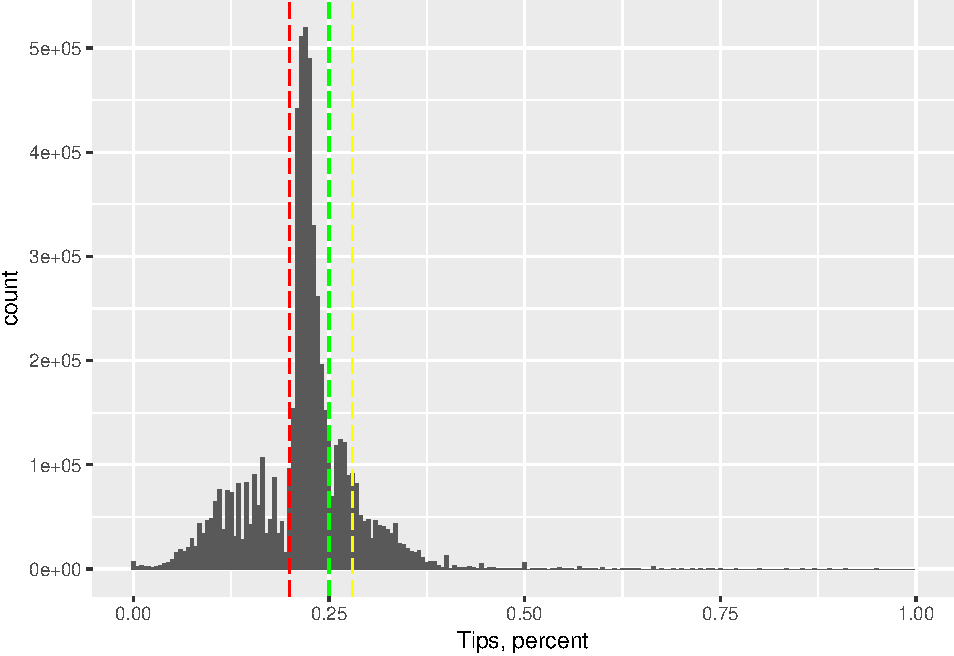
\includegraphics{thesis_files/figure-latex/unnamed-chunk-11-1.pdf}

One of the questions that I always wonder is whether longer trips result
in higher tip percent. It takes taxi drivers more time to complete
longer trips, so passengers might want to compensate taxi drivers more.
I personally pay higher percent of tips for longer rides, so I believe
trip distance has an impact on percentage of tips paid.
\begin{Shaded}
\begin{Highlighting}[]
\NormalTok{tip_distance <-}\StringTok{ }\KeywordTok{lm}\NormalTok{(tip_perct }\OperatorTok{~}\StringTok{ }\NormalTok{trip_distance, }\DataTypeTok{data =}\NormalTok{ yellow_}\FloatTok{2016.}\NormalTok{08_tip)}
\KeywordTok{summary}\NormalTok{(tip_distance)}
\end{Highlighting}
\end{Shaded}
\begin{verbatim}

Call:
lm(formula = tip_perct ~ trip_distance, data = yellow_2016.08_tip)

Residuals:
     Min       1Q   Median       3Q      Max 
-0.21887 -0.01889  0.00244  0.02682  0.77850 

Coefficients:
                Estimate Std. Error  t value Pr(>|t|)    
(Intercept)    2.189e-01  2.812e-05 7785.080   <2e-16 ***
trip_distance -4.146e-09  8.729e-09   -0.475    0.635    
---
Signif. codes:  0 '***' 0.001 '**' 0.01 '*' 0.05 '.' 0.1 ' ' 1

Residual standard error: 0.06938 on 6088289 degrees of freedom
Multiple R-squared:  3.706e-08, Adjusted R-squared:  -1.272e-07 
F-statistic: 0.2256 on 1 and 6088289 DF,  p-value: 0.6348
\end{verbatim}
Acoording to the simple linear regression result, trip distance does not
have significant impact on the percent of tips paid.

\subsection{Aggregated Zone-level Tip
Information}\label{aggregated-zone-level-tip-information}
\begin{Shaded}
\begin{Highlighting}[]
\KeywordTok{data}\NormalTok{(taxi_zone_lookup)}
\NormalTok{tip_region <-}\StringTok{ }\NormalTok{yellow_}\FloatTok{2016.}\NormalTok{08_tip  }\OperatorTok
\StringTok{  }\KeywordTok{group_by}\NormalTok{(PULocationID, DOLocationID) }\OperatorTok
\StringTok{  }\KeywordTok{summarise}\NormalTok{(}\DataTypeTok{avg_tip =} \KeywordTok{mean}\NormalTok{(tip_perct), }\DataTypeTok{trips =} \KeywordTok{n}\NormalTok{(),}
            \DataTypeTok{avg_dis =} \KeywordTok{mean}\NormalTok{(trip_distance)) }\OperatorTok
\StringTok{  }\KeywordTok{filter}\NormalTok{(trips }\OperatorTok{>}\StringTok{ }\DecValTok{10}\NormalTok{) }\OperatorTok
\StringTok{  }\KeywordTok{arrange}\NormalTok{(}\KeywordTok{desc}\NormalTok{(avg_tip)) }\OperatorTok
\StringTok{  }\KeywordTok{rename}\NormalTok{(}\DataTypeTok{LocationID =}\NormalTok{ PULocationID) }\OperatorTok
\StringTok{  }\KeywordTok{left_join}\NormalTok{(taxi_zone_lookup, }\DataTypeTok{by =} \StringTok{"LocationID"}\NormalTok{)}
\end{Highlighting}
\end{Shaded}
\begin{Shaded}
\begin{Highlighting}[]
\CommentTok{#zone}
\NormalTok{region_vis <-}\StringTok{ }\KeywordTok{ggplot}\NormalTok{(}\DataTypeTok{data =}\NormalTok{ tip_region, }\KeywordTok{aes}\NormalTok{(}\DataTypeTok{x =}\NormalTok{ avg_tip) ) }\OperatorTok{+}
\StringTok{  }\KeywordTok{xlab}\NormalTok{(}\StringTok{"Tips, percent"}\NormalTok{) }\OperatorTok{+}
\StringTok{  }\KeywordTok{geom_histogram}\NormalTok{(}\DataTypeTok{binwidth =} \FloatTok{0.005}\NormalTok{) }\OperatorTok{+}\StringTok{ }
\StringTok{  }\KeywordTok{geom_vline}\NormalTok{(}\DataTypeTok{xintercept =} \KeywordTok{c}\NormalTok{(}\FloatTok{0.20}\NormalTok{), }\DataTypeTok{col =} \StringTok{"red"}\NormalTok{,}\DataTypeTok{linetype =} \StringTok{"longdash"}\NormalTok{) }\OperatorTok{+}
\StringTok{  }\KeywordTok{geom_vline}\NormalTok{(}\DataTypeTok{xintercept =} \KeywordTok{c}\NormalTok{(}\FloatTok{0.25}\NormalTok{), }\DataTypeTok{col =} \StringTok{"green"}\NormalTok{,}\DataTypeTok{linetype =} \StringTok{"longdash"}\NormalTok{) }\OperatorTok{+}
\StringTok{  }\KeywordTok{geom_vline}\NormalTok{(}\DataTypeTok{xintercept =} \KeywordTok{c}\NormalTok{(}\FloatTok{0.28}\NormalTok{), }\DataTypeTok{col =} \StringTok{"yellow"}\NormalTok{,}\DataTypeTok{linetype =} \StringTok{"longdash"}\NormalTok{) }\OperatorTok{+}\StringTok{ }
\StringTok{  }\KeywordTok{scale_x_continuous}\NormalTok{(}\DataTypeTok{limits =} \KeywordTok{c}\NormalTok{(}\DecValTok{0}\NormalTok{, }\FloatTok{0.5}\NormalTok{))}
\NormalTok{region_vis}
\end{Highlighting}
\end{Shaded}
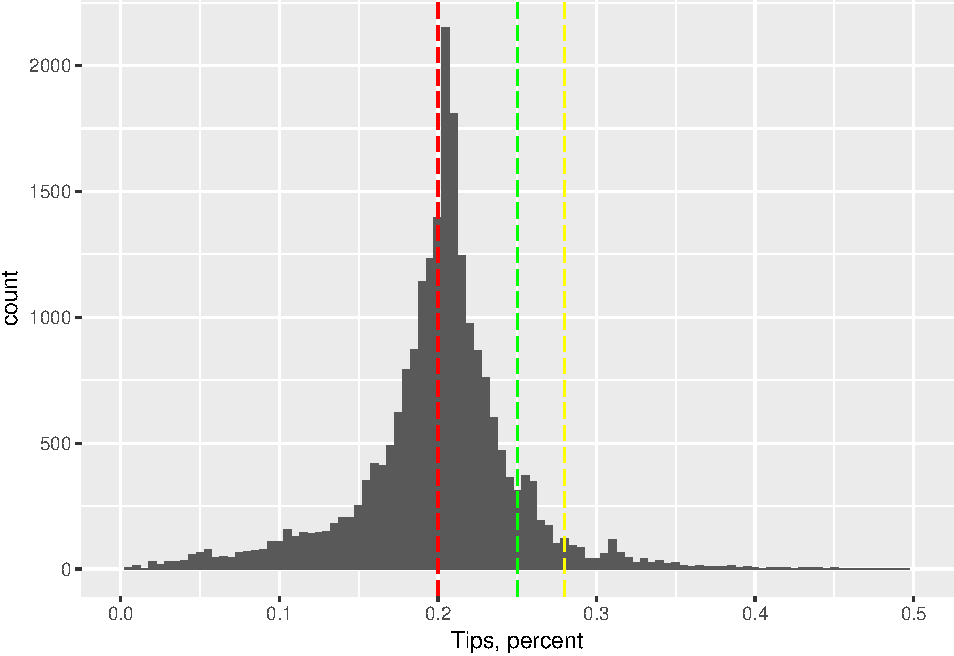
\includegraphics{thesis_files/figure-latex/unnamed-chunk-14-1.pdf}
\begin{Shaded}
\begin{Highlighting}[]
\NormalTok{tip_pickup <-}\StringTok{ }\NormalTok{tip_region }\OperatorTok
\StringTok{  }\KeywordTok{group_by}\NormalTok{(LocationID) }\OperatorTok
\StringTok{  }\KeywordTok{summarise}\NormalTok{(}\DataTypeTok{avg_tip =} \KeywordTok{mean}\NormalTok{(avg_tip), }\DataTypeTok{num_trips=}\KeywordTok{sum}\NormalTok{(trips)) }\OperatorTok
\StringTok{  }\KeywordTok{left_join}\NormalTok{(taxi_zone_lookup, }\DataTypeTok{by =} \StringTok{"LocationID"}\NormalTok{) }\OperatorTok
\StringTok{  }\KeywordTok{arrange}\NormalTok{(}\KeywordTok{desc}\NormalTok{(avg_tip)) }\OperatorTok
\StringTok{  }\KeywordTok{filter}\NormalTok{(Zone }\OperatorTok{!=}\StringTok{ "Unknown"}\NormalTok{)}

\NormalTok{region_pickup_vis <-}\StringTok{ }\NormalTok{region_vis }\OperatorTok\StringTok{ }\NormalTok{tip_pickup}
\NormalTok{region_pickup_vis}
\end{Highlighting}
\end{Shaded}
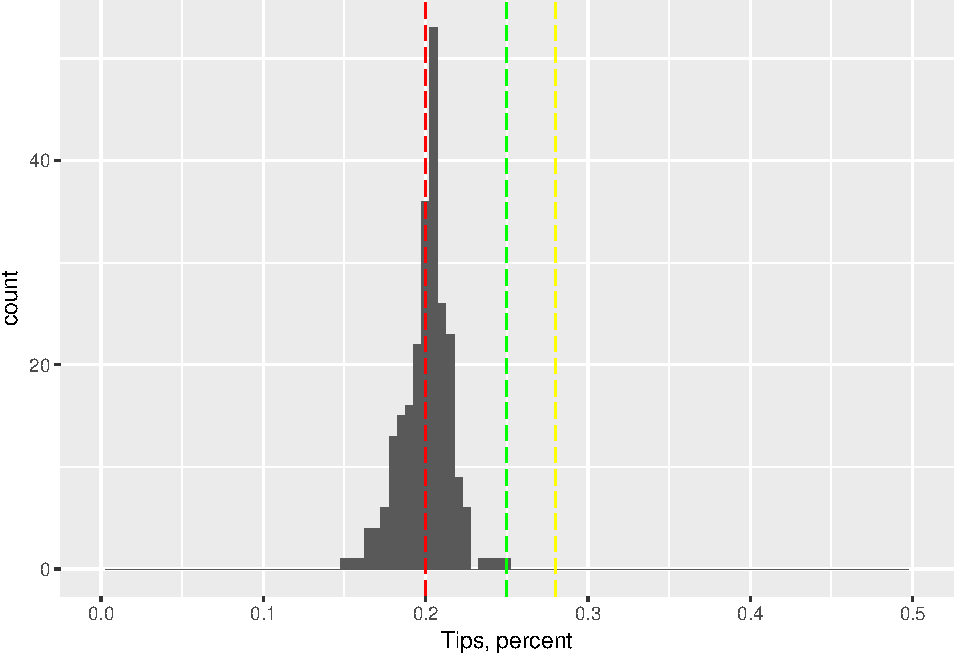
\includegraphics{thesis_files/figure-latex/unnamed-chunk-15-1.pdf}
\begin{Shaded}
\begin{Highlighting}[]
\NormalTok{tip_dropoff <-}\StringTok{ }\NormalTok{tip_region }\OperatorTok
\StringTok{  }\KeywordTok{group_by}\NormalTok{(DOLocationID) }\OperatorTok
\StringTok{  }\KeywordTok{summarise}\NormalTok{(}\DataTypeTok{avg_tip =} \KeywordTok{mean}\NormalTok{(avg_tip)) }\OperatorTok\StringTok{ }
\StringTok{  }\KeywordTok{rename}\NormalTok{(}\DataTypeTok{LocationID =}\NormalTok{ DOLocationID) }\OperatorTok
\StringTok{  }\KeywordTok{left_join}\NormalTok{(taxi_zone_lookup, }\DataTypeTok{by =} \StringTok{"LocationID"}\NormalTok{)}

\NormalTok{region_dropoff_vis <-}\StringTok{ }\NormalTok{region_pickup_vis }\OperatorTok\StringTok{ }\NormalTok{tip_dropoff}
\NormalTok{region_dropoff_vis}
\end{Highlighting}
\end{Shaded}
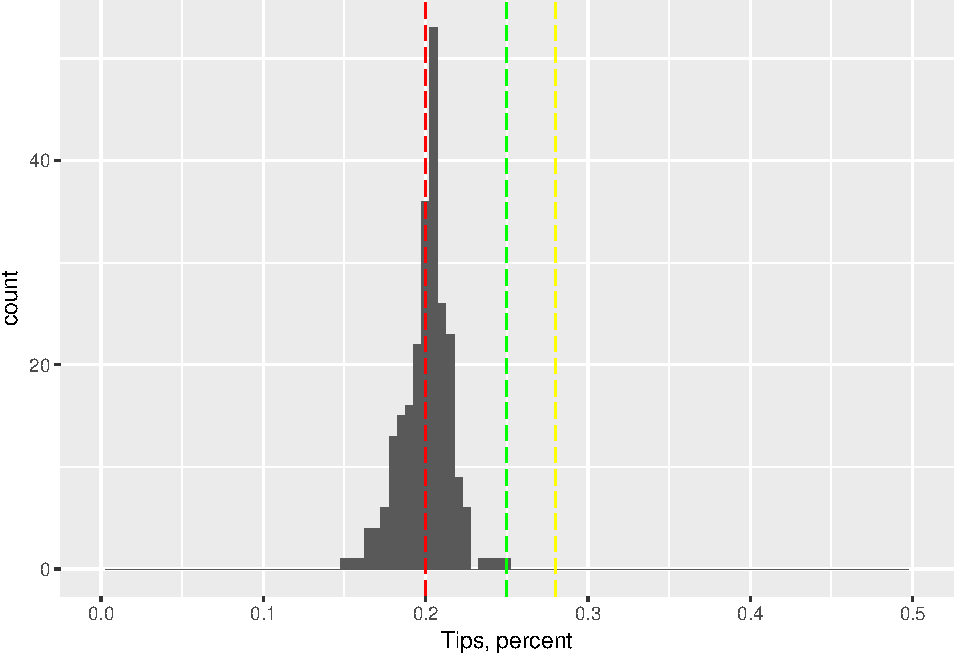
\includegraphics{thesis_files/figure-latex/unnamed-chunk-16-1.pdf}

Taxi drivers are required to be indifferent to where passengers are
going. Therefore, it makes more sense to investigate the average amount
of tips paid for each pick-up zone. What are the taxi zones that have
the highest tip percents?

Let's fist take a look at which zones have the highest number of
pickups.
\begin{Shaded}
\begin{Highlighting}[]
\KeywordTok{data}\NormalTok{(}\StringTok{"taxi_zones"}\NormalTok{)}
\KeywordTok{names}\NormalTok{(taxi_zones)}
\end{Highlighting}
\end{Shaded}
\begin{verbatim}
Loading required package: sp
\end{verbatim}
\begin{verbatim}
Warning: package 'sp' was built under R version 3.4.3
\end{verbatim}
\begin{verbatim}
[1] "OBJECTID"   "Shape_Leng" "Shape_Area" "zone"       "LocationID"
[6] "borough"   
\end{verbatim}
\begin{Shaded}
\begin{Highlighting}[]
\CommentTok{#names(taxi_zones)}
\NormalTok{newobj <-}\StringTok{ }\KeywordTok{merge}\NormalTok{(taxi_zones, tip_pickup, }\DataTypeTok{by.x =} \StringTok{"LocationID"}\NormalTok{, }\DataTypeTok{by.y =} \StringTok{"LocationID"}\NormalTok{)}
\KeywordTok{library}\NormalTok{(RColorBrewer)}
\NormalTok{cols <-}\StringTok{ }\KeywordTok{brewer.pal}\NormalTok{(}\DataTypeTok{n =} \DecValTok{4}\NormalTok{, }\DataTypeTok{name =} \StringTok{"Greys"}\NormalTok{)}
\NormalTok{lcols <-}\StringTok{ }\KeywordTok{cut}\NormalTok{(newobj}\OperatorTok{$}\NormalTok{num_trips,}
             \DataTypeTok{breaks =} \KeywordTok{quantile}\NormalTok{(newobj}\OperatorTok{$}\NormalTok{num_trips, }\DataTypeTok{na.rm =} \OtherTok{TRUE}\NormalTok{),}
             \DataTypeTok{labels =}\NormalTok{ cols)}
\KeywordTok{plot}\NormalTok{(newobj, }\DataTypeTok{col =} \KeywordTok{as.character}\NormalTok{(lcols))}
\end{Highlighting}
\end{Shaded}
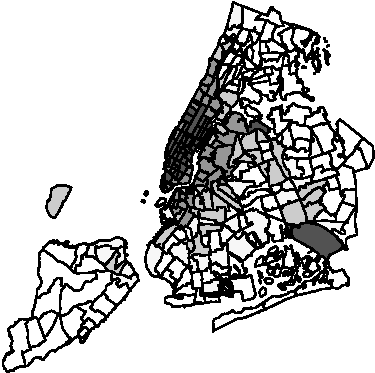
\includegraphics{thesis_files/figure-latex/unnamed-chunk-17-1.pdf}

\subsection{What are the zones with the highest percent
?}\label{what-are-the-zones-with-the-highest-percent}
\begin{Shaded}
\begin{Highlighting}[]
\CommentTok{#pick a threshold for the cutoff of number of trips}
\NormalTok{pickup_zone_}\DecValTok{1000}\NormalTok{ <-}\StringTok{ }\NormalTok{tip_pickup }\OperatorTok
\StringTok{  }\KeywordTok{filter}\NormalTok{(num_trips }\OperatorTok{>=}\StringTok{ }\DecValTok{1000}\NormalTok{) }\OperatorTok
\StringTok{  }\KeywordTok{arrange}\NormalTok{(}\KeywordTok{desc}\NormalTok{(avg_tip))}

\KeywordTok{library}\NormalTok{(knitr)}
\KeywordTok{kable}\NormalTok{(pickup_zone_}\DecValTok{1000}\NormalTok{[}\DecValTok{1}\OperatorTok{:}\DecValTok{10}\NormalTok{,}\DecValTok{2}\OperatorTok{:}\DecValTok{5}\NormalTok{], }\DataTypeTok{caption =} \StringTok{"Taxi zone with the highest tip percent, threshold = 1000"}\NormalTok{)}
\end{Highlighting}
\end{Shaded}
\begin{table}

\caption{\label{tab:unnamed-chunk-18}Taxi zone with the highest tip percent, threshold = 1000}
\centering
\begin{tabular}[t]{r|r|l|l}
\hline
avg\_tip & num\_trips & Borough & Zone\\
\hline
0.2220842 & 1514 & Brooklyn & Prospect Heights\\
\hline
0.2209707 & 1890 & Brooklyn & Bushwick South\\
\hline
0.2203979 & 1049 & Brooklyn & Crown Heights North\\
\hline
0.2203508 & 1812 & Brooklyn & Clinton Hill\\
\hline
0.2202720 & 2637 & Queens & Steinway\\
\hline
0.2196133 & 1177 & Brooklyn & Bedford\\
\hline
0.2189780 & 3321 & Brooklyn & Carroll Gardens\\
\hline
0.2148377 & 3429 & Brooklyn & Greenpoint\\
\hline
0.2143333 & 5566 & Queens & Long Island City/Hunters Point\\
\hline
0.2137938 & 4234 & Brooklyn & East Williamsburg\\
\hline
\end{tabular}
\end{table}
If we focus on the pick-up zones that have more than 10000 trips per
month, then we observe that all pick-up zones that have the highest
percent tips are in Manhattan besides LaGuardia Airport.
\begin{Shaded}
\begin{Highlighting}[]
\CommentTok{#pick a threshold for the cutoff of number of trips}
\NormalTok{pickup_zone_}\DecValTok{10000}\NormalTok{ <-}\StringTok{ }\NormalTok{tip_pickup }\OperatorTok
\StringTok{  }\KeywordTok{filter}\NormalTok{(num_trips }\OperatorTok{>=}\StringTok{ }\DecValTok{10000}\NormalTok{) }\OperatorTok
\StringTok{  }\KeywordTok{arrange}\NormalTok{(}\KeywordTok{desc}\NormalTok{(avg_tip))}
\KeywordTok{kable}\NormalTok{(pickup_zone_}\DecValTok{10000}\NormalTok{[}\DecValTok{1}\OperatorTok{:}\DecValTok{10}\NormalTok{,}\DecValTok{2}\OperatorTok{:}\DecValTok{5}\NormalTok{], }\DataTypeTok{caption =} \StringTok{"Taxi zone with the highest tip percent, threshold = 10000"}\NormalTok{)}
\end{Highlighting}
\end{Shaded}
\begin{table}

\caption{\label{tab:unnamed-chunk-19}Taxi zone with the highest tip percent, threshold = 10000}
\centering
\begin{tabular}[t]{r|r|l|l}
\hline
avg\_tip & num\_trips & Borough & Zone\\
\hline
0.2111362 & 39854 & Manhattan & Hudson Sq\\
\hline
0.2100087 & 224163 & Manhattan & Midtown East\\
\hline
0.2089467 & 63884 & Manhattan & Central Park\\
\hline
0.2087323 & 177105 & Queens & LaGuardia Airport\\
\hline
0.2085443 & 107154 & Manhattan & Greenwich Village North\\
\hline
0.2076574 & 33450 & Manhattan & World Trade Center\\
\hline
0.2076139 & 88966 & Manhattan & UN/Turtle Bay South\\
\hline
0.2075438 & 213399 & Manhattan & Penn Station/Madison Sq West\\
\hline
0.2073151 & 27055 & Manhattan & Financial District South\\
\hline
0.2064646 & 56759 & Manhattan & SoHo\\
\hline
\end{tabular}
\end{table}
\subsection{Do taxi drivers go to zones that offer high
tips?}\label{do-taxi-drivers-go-to-zones-that-offer-high-tips}

Pick-up zones with higher tips should attract more taxi drivers.
\begin{Shaded}
\begin{Highlighting}[]
\NormalTok{tip_region}\OperatorTok{$}\NormalTok{LocationID <-}\StringTok{ }\KeywordTok{as.character}\NormalTok{(tip_region}\OperatorTok{$}\NormalTok{LocationID)}
\NormalTok{tip_pickup}\OperatorTok{$}\NormalTok{LocationID <-}\StringTok{ }\KeywordTok{as.character}\NormalTok{(tip_pickup}\OperatorTok{$}\NormalTok{LocationID)}
\NormalTok{tip_and_trip_}\DecValTok{1}\NormalTok{ <-}\StringTok{ }\KeywordTok{lm}\NormalTok{(trips }\OperatorTok{~}\StringTok{ }\NormalTok{avg_tip }\OperatorTok{+}\StringTok{ }\NormalTok{LocationID, }\DataTypeTok{data =}\NormalTok{ tip_region)}
\KeywordTok{summary}\NormalTok{(tip_and_trip_}\DecValTok{1}\NormalTok{)}
\end{Highlighting}
\end{Shaded}
\begin{verbatim}

Call:
lm(formula = trips ~ avg_tip + LocationID, data = tip_region)

Residuals:
   Min     1Q Median     3Q    Max 
 -3780   -663   -183    246  62515 

Coefficients:
              Estimate Std. Error t value Pr(>|t|)    
(Intercept)   -2907.26    1456.57  -1.996   0.0460 *  
avg_tip       18382.03     643.53  28.564   <2e-16 ***
LocationID10   -936.47    1471.76  -0.636   0.5246    
LocationID100  -146.65    1456.66  -0.101   0.9198    
LocationID106 -1327.88    1478.24  -0.898   0.3691    
LocationID107   367.36    1457.42   0.252   0.8010    
LocationID112  -990.71    1463.11  -0.677   0.4983    
LocationID113   -75.78    1458.00  -0.052   0.9586    
LocationID114  -151.25    1457.84  -0.104   0.9174    
LocationID115  -932.89    2053.75  -0.454   0.6497    
LocationID116  -545.87    1464.83  -0.373   0.7094    
LocationID117 -1355.28    2053.90  -0.660   0.5094    
LocationID12   -913.56    1464.52  -0.624   0.5328    
LocationID125  -594.29    1459.17  -0.407   0.6838    
LocationID127 -1036.80    1523.19  -0.681   0.4961    
LocationID129  -862.22    1478.89  -0.583   0.5599    
LocationID13   -236.51    1458.24  -0.162   0.8712    
LocationID130  -801.18    1523.08  -0.526   0.5989    
LocationID132   -41.13    1455.22  -0.028   0.9775    
LocationID133 -1390.30    1623.97  -0.856   0.3920    
LocationID134 -1464.23    1677.23  -0.873   0.3827    
LocationID135 -4184.09    2058.02  -2.033   0.0421 *  
LocationID137  -185.17    1457.69  -0.127   0.8989    
LocationID138  -146.01    1455.46  -0.100   0.9201    
LocationID14  -1130.61    1778.69  -0.636   0.5250    
LocationID140    68.23    1457.41   0.047   0.9627    
LocationID141   232.75    1457.51   0.160   0.8731    
LocationID142   354.11    1457.96   0.243   0.8081    
LocationID143   -76.35    1459.87  -0.052   0.9583    
LocationID144  -233.85    1458.16  -0.160   0.8726    
LocationID145  -967.14    1460.82  -0.662   0.5080    
LocationID146  -693.04    1462.82  -0.474   0.6357    
LocationID148   -16.40    1456.93  -0.011   0.9910    
LocationID151  -160.33    1460.48  -0.110   0.9126    
LocationID152  -613.12    1466.90  -0.418   0.6760    
LocationID157  -921.67    2053.70  -0.449   0.6536    
LocationID158   -41.50    1458.24  -0.028   0.9773    
LocationID159 -1560.66    2054.04  -0.760   0.4474    
LocationID161   575.57    1456.82   0.395   0.6928    
LocationID162   350.15    1456.48   0.240   0.8100    
LocationID163   266.21    1457.50   0.183   0.8551    
LocationID164   155.58    1456.71   0.107   0.9149    
LocationID165 -2688.69    2055.25  -1.308   0.1908    
LocationID166  -555.16    1461.49  -0.380   0.7041    
LocationID168 -1234.45    1530.99  -0.806   0.4201    
LocationID17  -1090.44    1476.37  -0.739   0.4602    
LocationID170   415.75    1456.42   0.285   0.7753    
LocationID177 -1538.40    2054.03  -0.749   0.4539    
LocationID178  -445.39    2053.60  -0.217   0.8283    
LocationID179  -834.77    1469.84  -0.568   0.5701    
LocationID181  -886.06    1459.97  -0.607   0.5439    
LocationID186   347.47    1456.51   0.239   0.8114    
LocationID188 -1101.31    1516.92  -0.726   0.4678    
LocationID189 -1135.25    1471.38  -0.772   0.4404    
LocationID190 -1267.45    1591.05  -0.797   0.4257    
LocationID193  -918.34    1479.93  -0.621   0.5349    
LocationID194 -1070.92    1540.42  -0.695   0.4869    
LocationID195 -1280.82    1568.81  -0.816   0.4143    
LocationID196 -1132.43    1552.63  -0.729   0.4658    
LocationID197  -872.05    1778.57  -0.490   0.6239    
LocationID198 -1965.61    1677.73  -1.172   0.2414    
LocationID200 -1357.03    2053.91  -0.661   0.5088    
LocationID202 -1286.33    1623.87  -0.792   0.4283    
LocationID206 -1097.95    2053.77  -0.535   0.5929    
LocationID209  -727.16    1459.76  -0.498   0.6184    
LocationID210 -2751.74    2055.35  -1.339   0.1807    
LocationID211  -390.09    1458.59  -0.267   0.7891    
LocationID215  -754.50    1516.75  -0.497   0.6189    
LocationID216  -758.87    1676.84  -0.453   0.6509    
LocationID217 -1072.02    1530.88  -0.700   0.4838    
LocationID219  -689.67    1676.80  -0.411   0.6809    
LocationID220 -2136.47    2054.56  -1.040   0.2984    
LocationID221  -834.38    2053.69  -0.406   0.6845    
LocationID223 -1089.04    1466.82  -0.742   0.4578    
LocationID224  -472.24    1460.49  -0.323   0.7464    
LocationID225 -1284.59    1503.46  -0.854   0.3929    
LocationID226  -647.57    1460.79  -0.443   0.6576    
LocationID228 -1331.63    1517.09  -0.878   0.3801    
LocationID229    22.10    1457.62   0.015   0.9879    
LocationID230   129.93    1456.52   0.089   0.9289    
LocationID231    37.85    1457.24   0.026   0.9793    
LocationID232  -709.19    1459.45  -0.486   0.6270    
LocationID233  -224.75    1457.82  -0.154   0.8775    
LocationID234   657.47    1457.03   0.451   0.6518    
LocationID236   522.15    1457.81   0.358   0.7202    
LocationID237   687.51    1457.72   0.472   0.6372    
LocationID238    85.83    1458.25   0.059   0.9531    
LocationID239   267.90    1458.00   0.184   0.8542    
LocationID24   -575.82    1463.15  -0.394   0.6939    
LocationID243  -776.99    1486.37  -0.523   0.6012    
LocationID244  -563.98    1463.81  -0.385   0.7000    
LocationID245 -1055.00    2053.76  -0.514   0.6075    
LocationID246   -28.13    1458.16  -0.019   0.9846    
LocationID247 -1116.20    1540.46  -0.725   0.4687    
LocationID249   183.07    1457.44   0.126   0.9000    
LocationID25   -925.19    1461.22  -0.633   0.5266    
LocationID255  -712.61    1459.30  -0.488   0.6253    
LocationID256  -730.24    1460.07  -0.500   0.6170    
LocationID257 -1384.43    1677.16  -0.825   0.4091    
LocationID26  -1078.96    2053.76  -0.525   0.5993    
LocationID260  -599.78    1470.18  -0.408   0.6833    
LocationID261  -637.95    1458.13  -0.438   0.6618    
LocationID262  -163.52    1458.97  -0.112   0.9108    
LocationID263    45.49    1457.67   0.031   0.9751    
LocationID264  -248.23    1459.69  -0.170   0.8650    
LocationID265  -488.28    1590.89  -0.307   0.7589    
LocationID28  -1056.99    1676.94  -0.630   0.5285    
LocationID33   -882.15    1460.78  -0.604   0.5459    
LocationID34  -1406.30    1591.15  -0.884   0.3768    
LocationID35  -1293.82    2053.87  -0.630   0.5287    
LocationID36  -1152.73    1494.51  -0.771   0.4405    
LocationID37  -1100.63    1472.98  -0.747   0.4550    
LocationID38   -907.22    2053.69  -0.442   0.6587    
LocationID39  -1458.54    2053.98  -0.710   0.4777    
LocationID4    -606.70    1459.29  -0.416   0.6776    
LocationID40  -1066.91    1463.49  -0.729   0.4660    
LocationID41   -519.09    1462.81  -0.355   0.7227    
LocationID42   -575.20    1465.29  -0.393   0.6947    
LocationID43   -307.29    1459.36  -0.211   0.8332    
LocationID45   -730.91    1459.53  -0.501   0.6165    
LocationID48    319.92    1456.55   0.220   0.8262    
LocationID49  -1095.55    1471.36  -0.745   0.4565    
LocationID50   -363.85    1458.10  -0.250   0.8030    
LocationID52   -930.55    1462.76  -0.636   0.5247    
LocationID54  -1667.06    1540.91  -1.082   0.2793    
LocationID56   -961.27    2053.73  -0.468   0.6398    
LocationID6    -972.02    2053.72  -0.473   0.6360    
LocationID61  -1109.13    1476.38  -0.751   0.4525    
LocationID62  -1391.55    1591.14  -0.875   0.3818    
LocationID65   -734.58    1459.59  -0.503   0.6148    
LocationID66   -858.00    1463.19  -0.586   0.5576    
LocationID68    270.91    1457.16   0.186   0.8525    
LocationID69  -1571.95    2054.06  -0.765   0.4441    
LocationID7    -753.88    1461.49  -0.516   0.6060    
LocationID70  -1311.82    1494.61  -0.878   0.3801    
LocationID74   -517.69    1461.93  -0.354   0.7233    
LocationID75   -302.63    1459.76  -0.207   0.8358    
LocationID76  -1424.36    2053.96  -0.693   0.4880    
LocationID77  -1579.84    2054.06  -0.769   0.4418    
LocationID79    517.61    1456.75   0.355   0.7224    
LocationID8    -792.30    2053.66  -0.386   0.6997    
LocationID80   -960.44    1462.94  -0.657   0.5115    
LocationID82  -1052.65    1494.43  -0.704   0.4812    
LocationID83   -982.97    1540.37  -0.638   0.5234    
LocationID87   -390.35    1457.74  -0.268   0.7889    
LocationID88   -670.38    1458.49  -0.460   0.6458    
LocationID89   -997.81    1516.87  -0.658   0.5107    
LocationID9   -1433.27    2053.96  -0.698   0.4853    
LocationID90    157.84    1457.70   0.108   0.9138    
LocationID91    323.71    1778.61   0.182   0.8556    
LocationID92   -175.80    1778.47  -0.099   0.9213    
LocationID93  -1127.50    1479.02  -0.762   0.4459    
LocationID95  -1065.11    1497.03  -0.711   0.4768    
LocationID97   -844.35    1460.75  -0.578   0.5633    
---
Signif. codes:  0 '***' 0.001 '**' 0.01 '*' 0.05 '.' 0.1 ' ' 1

Residual standard error: 1452 on 9499 degrees of freedom
Multiple R-squared:  0.1573,    Adjusted R-squared:  0.1437 
F-statistic: 11.59 on 153 and 9499 DF,  p-value: < 2.2e-16
\end{verbatim}
Each one percent increase in tips is associated with 18382.03 increase
in the number of trips, controlling the pick-up zone.

\subsection{Which pick-up zone has the highest price per
minute}\label{which-pick-up-zone-has-the-highest-price-per-minute}

estmate slow traffic time

\section{New York City Taxi Consumer}\label{new-york-city-taxi-consumer}

\subsection{Does taxi fare change through time? Is taxi ride becoming
more
expensive?}\label{does-taxi-fare-change-through-time-is-taxi-ride-becoming-more-expensive}

\section{New York City Taxi Fare \& Limousine
Commission}\label{new-york-city-taxi-fare-limousine-commission}

\subsection{Should there be a flat rate between Manhattan and the JFK
Airport?}\label{should-there-be-a-flat-rate-between-manhattan-and-the-jfk-airport}

\subsubsection{People in Manhattan benefit from the \$52 flat
rate.}\label{people-in-manhattan-benefit-from-the-52-flat-rate.}

Why is there a flat rate to and from JFK airport and any location in
Manhattan? Why is the flat rate \$52? Does TLC make profit from the \$52
flat rate? Does \$52 reduce the cogestion on the road to JFK airport and
make taking a train a more preferable choice?

If there is no flat rate between JFK and Manhattan,
\begin{Shaded}
\begin{Highlighting}[]
\NormalTok{jfk_trip <-}\StringTok{ }\NormalTok{dataset }\OperatorTok
\StringTok{  }\KeywordTok{filter}\NormalTok{(RatecodeID }\OperatorTok{==}\StringTok{ }\DecValTok{2}\NormalTok{) }\OperatorTok
\StringTok{  }\KeywordTok{filter}\NormalTok{(payment_type }\OperatorTok{!=}\StringTok{ }\DecValTok{3}\NormalTok{) }\OperatorTok
\StringTok{  }\KeywordTok{filter}\NormalTok{(trip_distance }\OperatorTok{>}\StringTok{ }\DecValTok{0}\NormalTok{) }\OperatorTok
\StringTok{  }\KeywordTok{filter}\NormalTok{(fare_amount }\OperatorTok{>}\StringTok{ }\DecValTok{0}\NormalTok{) }\OperatorTok
\StringTok{  }\KeywordTok{filter}\NormalTok{(PULocationID }\OperatorTok{!=}\StringTok{ }\NormalTok{DOLocationID) }\OperatorTok
\StringTok{  }\KeywordTok{mutate}\NormalTok{(}\DataTypeTok{est_fare =} \FloatTok{2.5} \OperatorTok{+}\StringTok{ }\FloatTok{0.5} \OperatorTok{*}\StringTok{ }\NormalTok{trip_distance }\OperatorTok{*}\StringTok{ }\DecValTok{5} \OperatorTok{+}\StringTok{ }\NormalTok{extra }\OperatorTok{+}\StringTok{ }
\StringTok{           }\NormalTok{improvement_surcharge }\OperatorTok{+}\StringTok{ }\NormalTok{mta_tax }\OperatorTok{+}\StringTok{ }\NormalTok{tolls_amount,}
         \DataTypeTok{est_diff =}\NormalTok{ est_fare }\OperatorTok{-}\StringTok{ }\NormalTok{fare_amount)}

\NormalTok{to_jfk <-}\StringTok{ }\NormalTok{jfk_trip }\OperatorTok
\StringTok{  }\KeywordTok{filter}\NormalTok{(DOLocationID }\OperatorTok{==}\StringTok{ }\DecValTok{132}\NormalTok{)}

\NormalTok{from_jfk <-}\StringTok{ }\NormalTok{jfk_trip }\OperatorTok
\StringTok{  }\KeywordTok{filter}\NormalTok{(PULocationID }\OperatorTok{==}\StringTok{ }\DecValTok{132}\NormalTok{)}
\end{Highlighting}
\end{Shaded}
\begin{Shaded}
\begin{Highlighting}[]
\NormalTok{to_jkf_zone <-}\StringTok{ }\NormalTok{to_jfk }\OperatorTok
\StringTok{  }\KeywordTok{group_by}\NormalTok{(PULocationID) }\OperatorTok
\StringTok{  }\KeywordTok{summarise}\NormalTok{(}\DataTypeTok{num_trips =} \KeywordTok{n}\NormalTok{(),}
            \DataTypeTok{avg_dis =} \KeywordTok{mean}\NormalTok{(trip_distance),}
            \DataTypeTok{avg_fare =} \KeywordTok{mean}\NormalTok{(est_fare))}

\NormalTok{to_jkf_fare <-}\StringTok{ }\KeywordTok{merge}\NormalTok{(taxi_zones, to_jkf_zone, }\DataTypeTok{by.x =} \StringTok{"LocationID"}\NormalTok{, }\DataTypeTok{by.y =} \StringTok{"PULocationID"}\NormalTok{)}

\NormalTok{cols <-}\StringTok{ }\KeywordTok{brewer.pal}\NormalTok{(}\DataTypeTok{n =} \DecValTok{4}\NormalTok{, }\DataTypeTok{name =} \StringTok{"Greys"}\NormalTok{)}
\NormalTok{lcols <-}\StringTok{ }\KeywordTok{cut}\NormalTok{(to_jkf_fare}\OperatorTok{$}\NormalTok{avg_fare,}
             \DataTypeTok{breaks =} \KeywordTok{quantile}\NormalTok{(to_jkf_fare}\OperatorTok{$}\NormalTok{avg_fare, }\DataTypeTok{na.rm =} \OtherTok{TRUE}\NormalTok{),}
             \DataTypeTok{labels =}\NormalTok{ cols)}
\KeywordTok{plot}\NormalTok{(to_jkf_fare, }\DataTypeTok{col =} \KeywordTok{as.character}\NormalTok{(lcols))}
\end{Highlighting}
\end{Shaded}
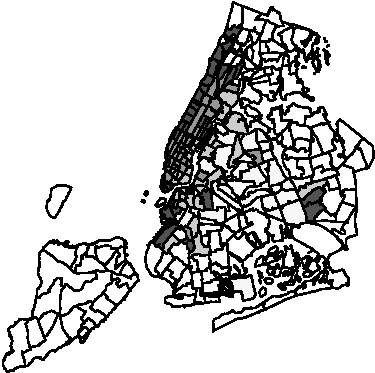
\includegraphics{thesis_files/figure-latex/unnamed-chunk-22-1.pdf}
\begin{Shaded}
\begin{Highlighting}[]
\NormalTok{to_jkf_zone_above <-}\StringTok{ }\NormalTok{to_jkf_zone }\OperatorTok
\StringTok{  }\KeywordTok{filter}\NormalTok{(avg_fare }\OperatorTok{>=}\StringTok{ }\DecValTok{52}\NormalTok{) }\OperatorTok
\StringTok{  }\KeywordTok{arrange}\NormalTok{(}\KeywordTok{desc}\NormalTok{(avg_fare))}
\KeywordTok{kable}\NormalTok{(to_jkf_zone_above[}\DecValTok{1}\OperatorTok{:}\DecValTok{10}\NormalTok{,], }\DataTypeTok{caption =} \StringTok{"Zones that woulde have paid more than $52"}\NormalTok{)}
\end{Highlighting}
\end{Shaded}
\textbackslash{}begin\{table\}

\textbackslash{}caption\{\label{tab:unnamed-chunk-23}Zones that woulde have
paid more than \$52\} \centering
\begin{tabular}[t]{r|r|r|r}
\hline
PULocationID & num\_trips & avg\_dis & avg\_fare\\
\hline
47 & 1 & 27.08000 & 76.54000\\
\hline
195 & 4 & 26.14000 & 74.19000\\
\hline
220 & 1 & 24.30000 & 69.59000\\
\hline
54 & 1 & 25.80000 & 67.80000\\
\hline
127 & 6 & 22.85833 & 65.06250\\
\hline
243 & 8 & 21.54250 & 63.82125\\
\hline
17 & 1 & 23.70000 & 62.55000\\
\hline
13 & 1266 & 22.09787 & 62.44055\\
\hline
244 & 74 & 20.42216 & 60.27892\\
\hline
133 & 1 & 18.74000 & 60.19000\\
\hline
\end{tabular}
\textbackslash{}end\{table\}

Imagine you are travelling to New York City and you do not know much
about the city. Travellers tend to gather around Mahanttan, and without
the flat rate, passengers would have paid more than \$52 to take a taxi
to go to the JFK Airport. The \$52 flat rate is nice for people who are
not very familiar with New York City, and it incentivize tourists to
take taxi to the JFK Airport. It also helps taxi drivers to get more
tips to JFK Airport.

\subsection{However, are taxi drivers happy with the flat
rate?}\label{however-are-taxi-drivers-happy-with-the-flat-rate}

What the expected fare from JKF Airport how much time it would take for
a cb driver to do a round trip

\chapter*{Conclusion}\label{conclusion}
\addcontentsline{toc}{chapter}{Conclusion}

\chapter{Future Research}\label{future-research}

For future study, I would love to investigate the sharp decline in the
consumption of NYC yellow cab after e-hail services were introduced into
the NYC ride-hail market. I also want to study what the impact of
introducing new GPS and entertainment system is on the number of rides.
The global product and marketing at Verifone, Jason Gross, said that,
``I like to say that we provide what Uber says it provides.'' With the
raised expectation among rides caused by Uber and Lyft, yellow taxi
industry need to respond quickly. How does the market react to the newly
installed entertainment system? Has the market share of yellow cab
rebounded since 2016? By looking into the patterns in market shares, it
might be possible for me to predict the future market share distribution
and find out what features of ride-hail transportation are the ones that
affect market share distribution the most.

\appendix

\chapter{The First Appendix}\label{the-first-appendix}

This first appendix includes all of the R chunks of code that were
hidden throughout the document (using the \texttt{include\ =\ FALSE}
chunk tag) to help with readibility and/or setup.

\textbf{In the main Rmd file}
\begin{Shaded}
\begin{Highlighting}[]
\CommentTok{# This chunk ensures that the thesisdown package is}
\CommentTok{# installed and loaded. This thesisdown package includes}
\CommentTok{# the template files for the thesis.}
\ControlFlowTok{if}\NormalTok{(}\OperatorTok{!}\KeywordTok{require}\NormalTok{(devtools))}
  \KeywordTok{install.packages}\NormalTok{(}\StringTok{"devtools"}\NormalTok{, }\DataTypeTok{repos =} \StringTok{"http://cran.rstudio.com"}\NormalTok{)}
\ControlFlowTok{if}\NormalTok{(}\OperatorTok{!}\KeywordTok{require}\NormalTok{(thesisdown))}
\NormalTok{  devtools}\OperatorTok{::}\KeywordTok{install_github}\NormalTok{(}\StringTok{"ismayc/thesisdown"}\NormalTok{)}
\KeywordTok{library}\NormalTok{(thesisdown)}
\end{Highlighting}
\end{Shaded}
\textbf{In Chapter \ref{ref-labels}:}

\chapter{The Second Appendix, for
Fun}\label{the-second-appendix-for-fun}

\backmatter

\chapter*{References}\label{references}
\addcontentsline{toc}{chapter}{References}

\markboth{References}{References}

\noindent

\setlength{\parindent}{-0.20in} \setlength{\leftskip}{0.20in}
\setlength{\parskip}{8pt}

\hypertarget{refs}{}
\hypertarget{ref-angel2000}{}
Angel, E. (2000). \emph{Interactive computer graphics : A top-down
approach with opengl}. Boston, MA: Addison Wesley Longman.

\hypertarget{ref-angel2001}{}
Angel, E. (2001a). \emph{Batch-file computer graphics : A bottom-up
approach with quicktime}. Boston, MA: Wesley Addison Longman.

\hypertarget{ref-angel2002a}{}
Angel, E. (2001b). \emph{Test second book by angel}. Boston, MA: Wesley
Addison Longman.


% Index?

\end{document}
